\chapter{Results}
\label{cha:res}

It is much harder to interpret the results of dynamic test than the results of quasi static tests. A quasi static test has a clearly defined point of failure and therefore a maximum strength. With enough data points a statistical model can be made to predict the average strength of a sample with the given composition. For dynamic tests defining a failure criteria is more complex. How much displacement is accepted? At what crack opening widths can the specimen no longer withstand the static load?

In order to analyse the test results, these questions had to be answered. To analyse and visualise the data several tools were used.

\section{Data Analysis Tools}

The program used for data analysis was written in Python 3. \autocite{python} Several modules were used: NumPy, SciPy, Pandas, adjust\_text and Seaborn. \autocite{numpy} \autocite{Scipy} \autocite{Pandas} \autocite{adjust_text} \autocite{seaborn}

Visualisations were made with Ti\textit{k}Z \autocite{Tikz}, Matplotlib \autocite{matplotlib} or Inkscape \autocite{Inkscape}. 

\section{Data Analysis Method}

The Python Code is accessible at https://github.com/Sevarina/master\_thesis.

The data was passed through a median filter before plotting. The graphs for each individual test can be found in the appendix.

\section{Sensor Failure}
\label{sec:exc}

The sensor array suffered several failures. See \autoref{tab:excl}. The loadcells failed for two reasons. For the first two tests the measurments they took are no usable and for 2019-05-06\_Rfrs\_75\_0,8 the connector of load cell 3 was damaged when positioning the sample and the load cell did not capture any data. The internal accelerometer failed only in the first two tests, again because the measurements are not usable. The laser sensor readings are very vulnerable to failure, especially before the reflective tape was applied. The high speed camera has several failure modes. For the first few tests it was not used yet and in later tests it was either out of focus, zoomed in too far or the video capture was not turned on. 

\begin{landscape}
\begin{table}
    \centering
\begin{tabular}{llllllp{2cm}p{2cm}}
\toprule
{} & Loadcells & Accelerometer & Laser sensor &  Cracks & High speed camera & Additional accelerometer vertical & Additional accelerometer horizontal \\
Name                          &           &               &              &         &                   &                                   &                                     \\
\midrule
2017-12-20\_Rfrs\_75\_1,8     &    faulty &        faulty &       faulty &  faulty &            faulty &                            faulty &                              faulty \\
2017-12-20\_Rfrs\_75\_3,5     &    faulty &        faulty &       faulty &  faulty &            faulty &                            faulty &                              faulty \\
2018-02-14\_Rfrs\_75\_0,5     &           &               &              &         &            faulty &                            faulty &                              faulty \\
2018-02-14\_Rfrs\_75\_1,0     &           &               &       faulty &         &            faulty &                            faulty &                              faulty \\
2018-11-09\_Rfrs\_75\_0,5     &           &               &       faulty &         &            faulty &                            faulty &                              faulty \\
2018-11-29\_Rfrs\_75\_1,0     &           &               &       faulty &         &                   &                            faulty &                              faulty \\
2018-12-04\_Rfrs\_50\_0,3     &           &               &       faulty &         &                   &                            faulty &                              faulty \\
2018-12-04\_Rfrs\_50\_0,3\_2  &           &               &              &         &                   &                            faulty &                              faulty \\
2018-12-04\_Rfrs\_50\_0,7     &           &               &       faulty &  faulty &            faulty &                            faulty &                              faulty \\
2018-12-10\_Rfrs\_100\_1,5    &           &               &              &         &                   &                            faulty &                              faulty \\
2018-12-10\_Rfrs\_100\_1,5\_2 &           &               &       faulty &         &                   &                            faulty &                              faulty \\
2018-12-10\_Rfrs\_100\_2,0    &           &               &       faulty &  faulty &            faulty &                            faulty &                              faulty \\
2019-02-20\_Rfrs\_75\_0,5     &           &               &              &         &            faulty &                                   &                              faulty \\
2019-02-20\_Rfrs\_75\_1,0     &           &               &       faulty &  faulty &            faulty &                                   &                              faulty \\
2019-04-03\_Rfrs\_75\_1,0     &           &               &       faulty &  faulty &            faulty &                            faulty &                              faulty \\
2019-04-16\_Rfrs\_75\_0,5     &    faulty &        faulty &              &         &                   &                                   &                                     \\
2019-05-06\_Rfrs\_75\_0,8     &    faulty &               &              &         &            faulty &                            faulty &                              faulty \\
2019-08-19\_Rfrs+t\_75\_1,0      &           &               &              &         &                   &                            faulty &                              faulty \\
2019-08-19\_Rfrs+t\_75\_1,0m2,0  &           &               &              &  faulty &            faulty &                            faulty &                              faulty \\
\bottomrule
\end{tabular}

\caption{Sensor failure for all tests}
    \label{tab:excl}
\end{table}
\end{landscape}

\begin{table}
    \centering
\begin{tabular}{lll}
\toprule
{} & Additional accelerometer vertical & Additional accelerometer horizontal \\
Name                          &                                   &                                     \\
\midrule
2017-12-20\_Rfrs\_75\_1,8     &                            faulty &                              faulty \\
2017-12-20\_Rfrs\_75\_3,5     &                            faulty &                              faulty \\
2018-02-14\_Rfrs\_75\_0,5     &                            faulty &                              faulty \\
2018-02-14\_Rfrs\_75\_1,0     &                            faulty &                              faulty \\
2018-11-09\_Rfrs\_75\_0,5     &                            faulty &                              faulty \\
2018-11-29\_Rfrs\_75\_1,0     &                            faulty &                              faulty \\
2018-12-04\_Rfrs\_50\_0,3     &                            faulty &                              faulty \\
2018-12-04\_Rfrs\_50\_0,3\_2  &                            faulty &                              faulty \\
2018-12-04\_Rfrs\_50\_0,7     &                            faulty &                              faulty \\
2018-12-10\_Rfrs\_100\_1,5    &                            faulty &                              faulty \\
2018-12-10\_Rfrs\_100\_1,5\_2 &                            faulty &                              faulty \\
2018-12-10\_Rfrs\_100\_2,0    &                            faulty &                              faulty \\
2019-02-20\_Rfrs\_75\_0,5     &                                   &                              faulty \\
2019-02-20\_Rfrs\_75\_1,0     &                                   &                              faulty \\
2019-04-03\_Rfrs\_75\_1,0     &                            faulty &                              faulty \\
2019-04-16\_Rfrs\_75\_0,5     &                                   &                                     \\
2019-05-06\_Rfrs\_75\_0,8     &                            faulty &                              faulty \\
\bottomrule
\end{tabular}

    \caption{Failure of additional accelerometers}
    \label{tab:accl_excl}
\end{table}

The additional accelerometer were only added into the array later but they failed a few times as well. See \autoref{tab:accl_excl}. The extra accelerometer failed for a few reasons. For the first measurement the the measuring range was too small. The acceleration exceeded the expectation. Later failures were either related to the data loggers battery or problems with gluing the metal plates on the sample. The sample 2019-04-03\_Rfrs\_75\_1,0 was used for presenting the general function of the test rig to the mining research and development department of LKAB and only the basic sensor array was used for this purpose.

The sample 2019-04-16\_Rfrs\_75\_0,5 used the 50 kg drop weight unlike the other tests. The resulting force and acceleration are very different from those of the other results. They were excluded so the interpolated curves would not be skewed by the outlier. The sensor data appears to be very sensitive to changes in the drop weight.

There are very few experiments where every sensor was working properly. This highlights the importance of a redundant sensor array.

A few changes were implemented to increase the reliability the sensor array.

\subsection{Increasing The Reliability of the Laser Sensor}

After the impact the sample cracks and it is clearly visible on the high speed camera that dust and small particles are expelled. These affect the laser sensor readings negatively. See \autoref{fig:laser}.
In \autoref{fig:laserperfect} a near perfect laser reading is displayed. Note the initial fast deformations, which reach an elastic maximum and then stabilize at the plastic post peak value. The distortions were removed in post - processing.
Compare it with \autoref{fig:goodlaser}. Again both the elastic deformation and the plastic post peak deformation are clearly visible, even if slightly distorted. The distortions were removed in post - processing.
Many of the readings looked more like \autoref{fig:badlaser}. Please note, that the panel did not break during the experiment.
Especially interesting is \autoref{fig:weirdlaser}. The diagonal lines in the reading are most likely caused by an ejected particle. The displacement measurement shows the position of the particle at any given point in time. With this information it is possible to  to calculate the ejection velocity: \( 2 \rfrac{m}{s}\) the drop weight had a velocity of \( 2,4 \rfrac{m}{s}\). 
The impact velocity of the drop weight is higher than then the ejection velocity of the particle. It might be interesting to use the high speed camera footage of other experiments to try and calculate the ejection velocity of other samples and see how it aligns with the impact velocity of the drop weight.
Another challenge with the laser sensor was that the laser beam is pointed at the center of the specimen. For the round samples the desired failure mode according to \textcite{c1550} is 3 or more radial cracks. This often causes the center to crack as well. 
For the square panels there was little data available on how the failure modes would look. The a priori idea was either cracks from corner to corner or cracks from the middle of the edges. Either way, the center was estimated to likely experience cracking in some of the cases. 
In those cases the laser does not only measure the displacement but includes a random error, the depth of the crack. To enhance understanding this problem is visualized in \autoref{fig:displace}. The dashed lines show the shape of the test panel before the test. \autoref{fig:ideallaser} displays the ideal situation of uncracked concrete. The laser hits the surface of the panel at its center point and provides an accurate measurement of the peak displacement. \autoref{fig:reallaser} on the right hand side shows the real conditions. The concrete panel has cracked under the applied impact load. The laser no longer hits the surface of the concrete but instead the inside of a crack. Therefore the measured displacement is no longer accurate but a random value. The situations depicted is an extreme case, where the displacement would appear to be negative. There were no such cases recorded during testing, It merely serves to illustrate the problem. 

\begin{landscape}
\begin{figure} [p!]
\centering 
\subcaptionbox{Idealized situation \label{fig:ideallaser}}
{
\begin{tikzpicture}
%laser hitting cracks ideal

\draw [dashed, gray] (0,3) -- (10,3)
coordinate [midway] (start)
(0,0) -- (10,0);

%upper arc
\draw (0,3) arc [radius = 28.8cm, start angle= -100, end angle= -80];
%\draw (5,2) coordinate (myNode);

%lower arc
\draw (0,0) arc [radius = 28.8cm, start angle= -100, end angle= -80]
coordinate [midway] (laserpoint);

%laser
\draw (5,-5) node [rectangle,draw] (laser) {Laser};
\draw [red,-{Latex[length=3mm, width=1mm]}] (laser) -- (laserpoint);


%coordinate [at end] (myEnd)
%-- (myNode) (10,0) arc [radius = 28.8cm, start angle = 280, delta angle= -8]
%-- (myNode)
%coordinate [near start] (fik);

%thought line
%\draw[dashed] (myEnd) arc [radius = 28.8cm, start angle= -92, delta angle= 4]
%coordinate [midway] (lowPoint);


\begin{comment}
\draw[red]
[{Latex[length=3mm, width=1mm]}-{Latex[length=3mm, width=1mm]}] (start) -- (myNode) 
node [near end, black,right] {measured displacement};
\draw [{Latex[length=3mm, width=1mm]}-{Latex[length=3mm, width=1mm]}] (myEnd) -- ++ (0,3.4) 
node [midway, black,left] {real displacement};
\end{comment}


\end{tikzpicture}
} 
\subcaptionbox{Real situation \label{fig:reallaser}} 
{
\begin{tikzpicture}
%laser hitting crack real

%original design
\draw [dashed, gray] (0,3) -- (10,3)
coordinate [midway] (start)
(0,0) -- (10,0);

%upper arc
\draw (0,3) arc [radius = 28.8cm, start angle= -100, end angle= -80];

\begin{comment}
\path (0,2.5) arc [radius = 28.8cm, start angle= -100, end angle= -94.9]
coordinate [at end] (11);
\path (0,2.5) arc [radius = 28.8cm, start angle= -100, end angle= -92.25]
coordinate [at end] (11a);
\path (0,2.5) arc [radius = 28.8cm, start angle= -100, end angle= -90]
coordinate [at end] (12);
\path (0,2.5) arc [radius = 28.8cm, start angle= -100, end angle= -87.75]
coordinate [at end] (13);
\path (0,2.5) arc [radius = 28.8cm, start angle= -100, end angle= -85.85]
coordinate [at end] (14);
\path (0,2.5) arc [radius = 28.8cm, start angle= -100, end angle= -83.6]
coordinate [at end] (15)
;
\end{comment}

\path (0,2.5) arc [radius = 28.8cm, start angle= -100, end angle= -94.2]
coordinate [at end] (11);
\path (0,2.5) arc [radius = 28.8cm, start angle= -100, end angle= -92]
coordinate [at end] (11a);
\path (0,2.5) arc [radius = 28.8cm, start angle= -100, end angle= -90]
coordinate [at end] (12);
\path (0,2.5) arc [radius = 28.8cm, start angle= -100, end angle= -88]
coordinate [at end] (13);
\path (0,2.5) arc [radius = 28.8cm, start angle= -100, end angle= -86.3]
coordinate [at end] (14);
\path (0,2.5) arc [radius = 28.8cm, start angle= -100, end angle= -84.3]
coordinate [at end] (15)
;

\draw (0,0) arc [radius = 28.8cm, start angle= -100, end angle= -95]
coordinate (1);
\path (1) arc [radius = 28.8cm, start angle= -95, end angle= -94.7]
coordinate (2);
\draw (2) arc [radius = 28.8cm, start angle= -94.7, end angle= -92.5]
coordinate (1a);
\path (1a) arc [radius = 28.8cm, start angle= -92.5, end angle= -92]
coordinate (2a);
\draw (2a) arc [radius = 28.8cm, start angle= -92, end angle= -90.5]
coordinate (3);
\path (3) arc [radius = 28.8cm, start angle= -90.5, end angle= -89.5]
coordinate (4);
\draw (4) arc [radius = 28.8cm, start angle= -89.5, end angle= -88]
coordinate (5);
\path (5) arc [radius = 28.8cm, start angle= -88, end angle= -87.5]
coordinate (6);
\draw (6) arc [radius = 28.8cm, start angle= -87.5, end angle= -86]
coordinate (7);
\path (7) arc [radius = 28.8cm, start angle= -86, end angle= -85.7]
coordinate (8);
\draw (8) arc [radius = 28.8cm, start angle= -85.7, end angle= -84]
coordinate (9);
\path (9) arc [radius = 28.8cm, start angle= -84, end angle= -83.2]
coordinate (10);
\draw (10) arc [radius = 28.8cm, start angle= -83.2, end angle= -80];

%lower arc
%\draw (0,0) arc [radius = 28.8cm, start angle= -100, end angle= -80];

\begin{comment}
coordinate [pos=0.3] (1)
coordinate [pos=0.32] (2)
coordinate [pos=0.42] (3)
coordinate [pos=0.44] (4)
coordinate [pos=0.49] (5)
coordinate [pos=0.51] (6)
coordinate [pos=0.55] (7)
coordinate [pos=0.57] (8)
coordinate [pos=0.59] (9)
coordinate [pos=0.61] (10);
% roots of the cracks
\end{comment}

\draw (1) -- (11) -- (2)
(3) -- (12) -- (4)
(5) -- (13) -- (6)
(7) -- (14) -- (8)
(9) -- (15) -- (10)
(1a) -- (11a) -- (2a)
node [midway] (laserpoint) {};


%laser
\draw (5,-5) node [rectangle,draw] (laser) {Laser};
\draw [red,-{Latex[length=3mm, width=1mm]}] (laser) -- (12);


%coordinate [at end] (myEnd)
%-- (myNode) (10,0) arc [radius = 28.8cm, start angle = 280, delta angle= -8]
%-- (myNode)
%coordinate [near start] (fik);

%thought line
%\draw[dashed] (myEnd) arc [radius = 28.8cm, start angle= -92, delta angle= 4]
%coordinate [midway] (lowPoint);

\end{tikzpicture}
}

\caption{Difference in displacement measurement considering ideal and real conditions}
\label{fig:displace} 
\end{figure}
\end{landscape}

\begin{figure} 
\centering
\subcaptionbox{A perfect laser reading\\ test 2018-12-10\_Rfrs\_100\_1,5 
\label{fig:laserperfect}} 
{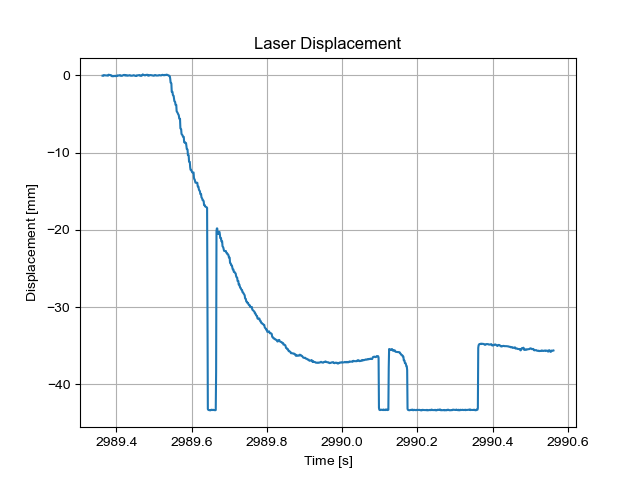
\includegraphics[width=0.45\linewidth]{pics/perfectlaser.png}} 
\subcaptionbox{A usable laser reading,\\test 2018-12-04\_Rfrs\_50\_0,3\_2 
\label{fig:goodlaser}}
{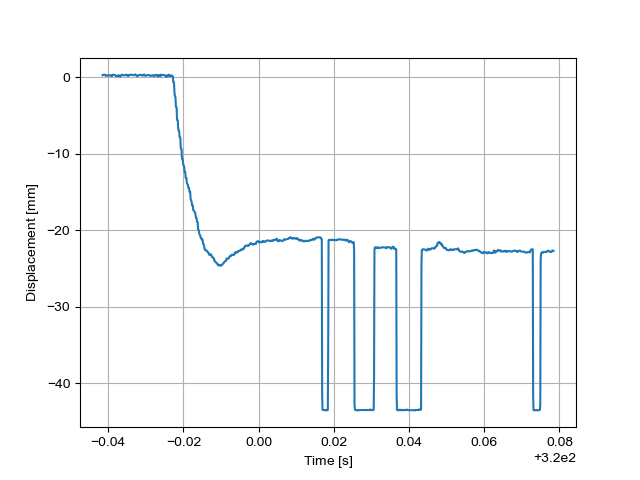
\includegraphics[width=0.45\linewidth]{pics/goodlaser.png}} 
\subcaptionbox{A bad laser reading,\\test 2018-11-09\_Rfrs\_70\_0,5 
\label{fig:badlaser}} 
{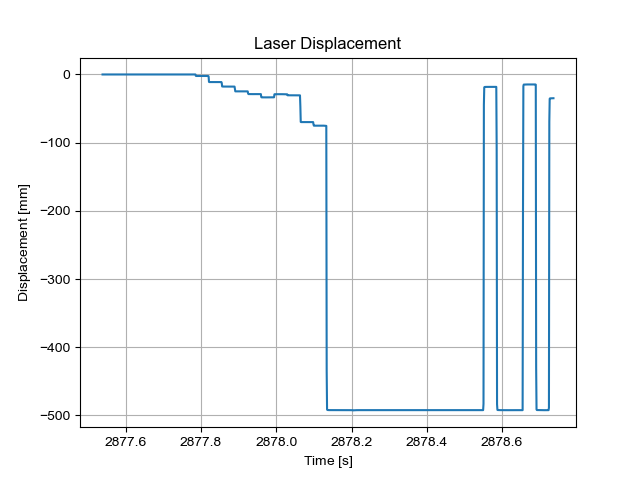
\includegraphics[width=0.45\linewidth]{pics/badlaser.png}} 
\subcaptionbox{An ejected particle (\(v = 2~\rfrac{m}{s}\)) caught in the beam,\\test 2018-12-04\_Rfrs\_50\_0,3 
\label{fig:weirdlaser}}
{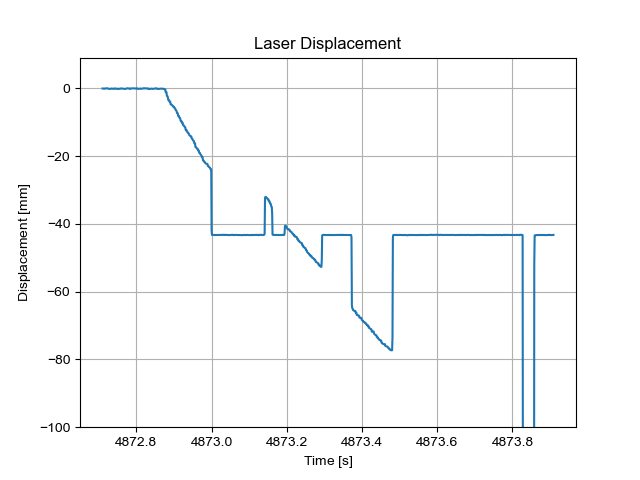
\includegraphics[width=0.45\linewidth]{pics/weirdlaser.png}} 
\caption{Problems with laser sensor readings} \label{fig:laser} 
\end{figure}

\begin{figure} 
\centering
\subcaptionbox{Parallel tape after a test
    \label{fig:riptape}}{
    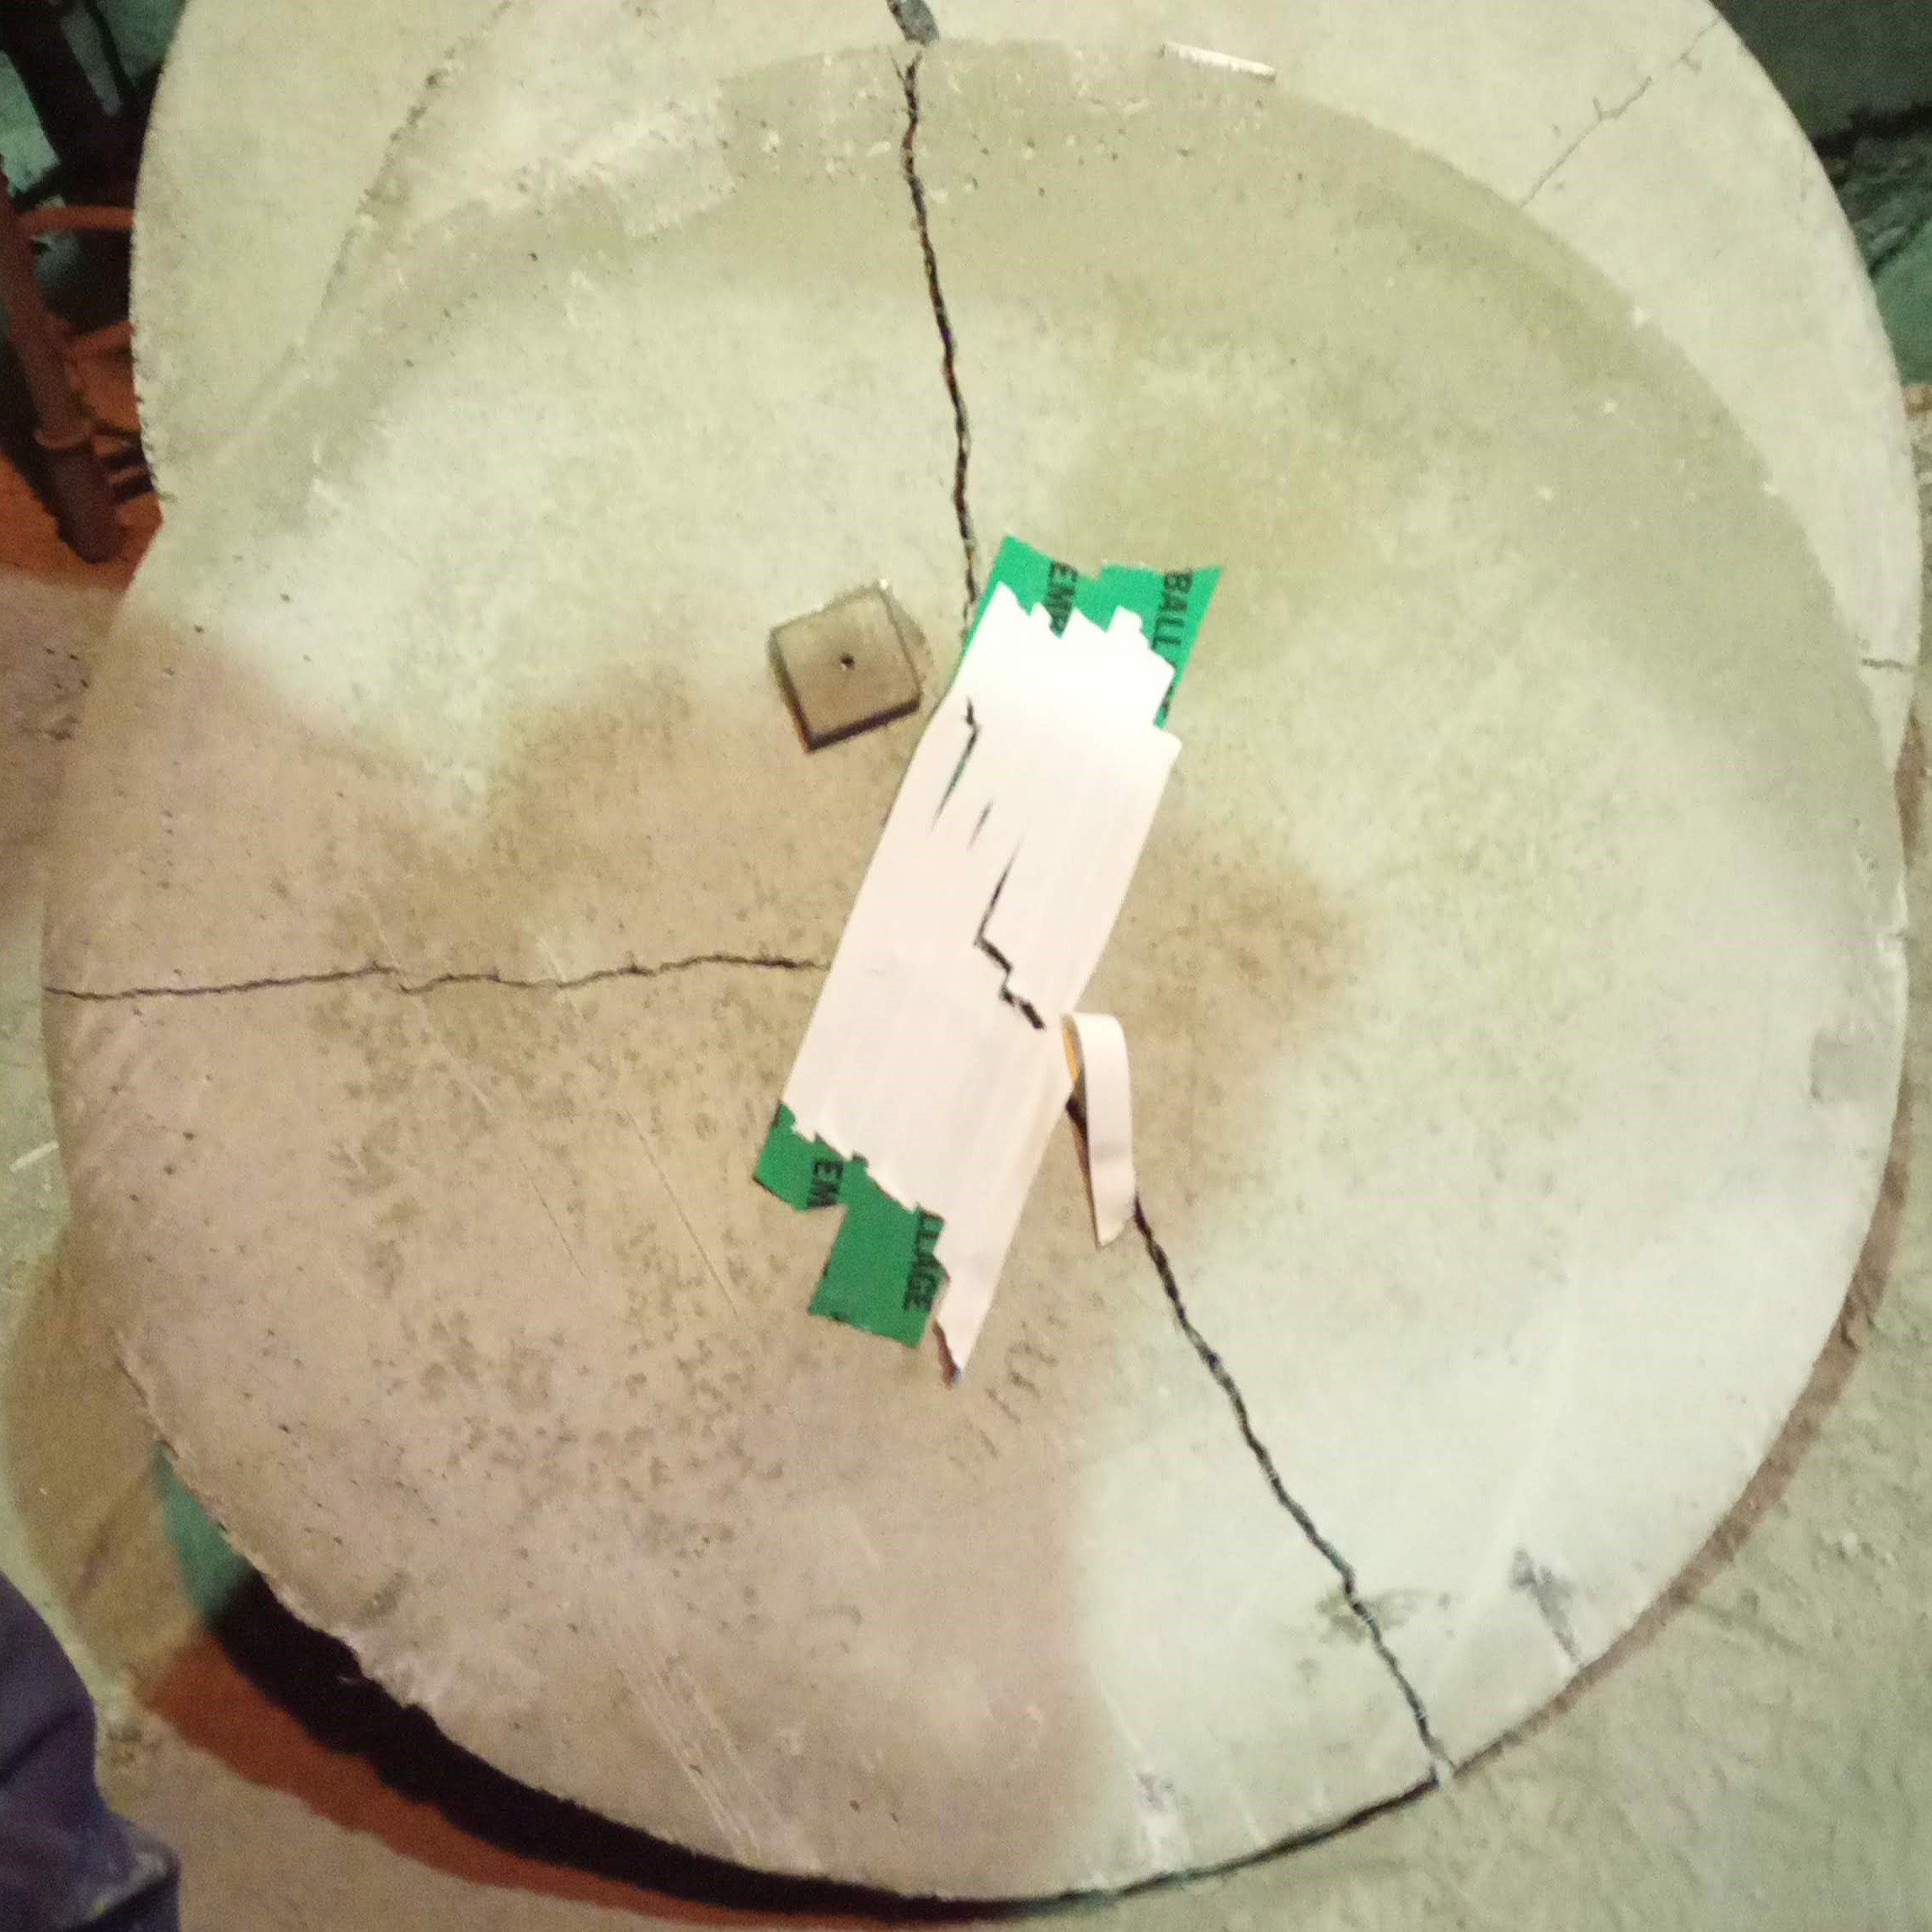
\includegraphics[width=0.45\linewidth]{pics/parallel.jpg}}
\subcaptionbox{Basket weave tape after a test\label{fig:tape}}{
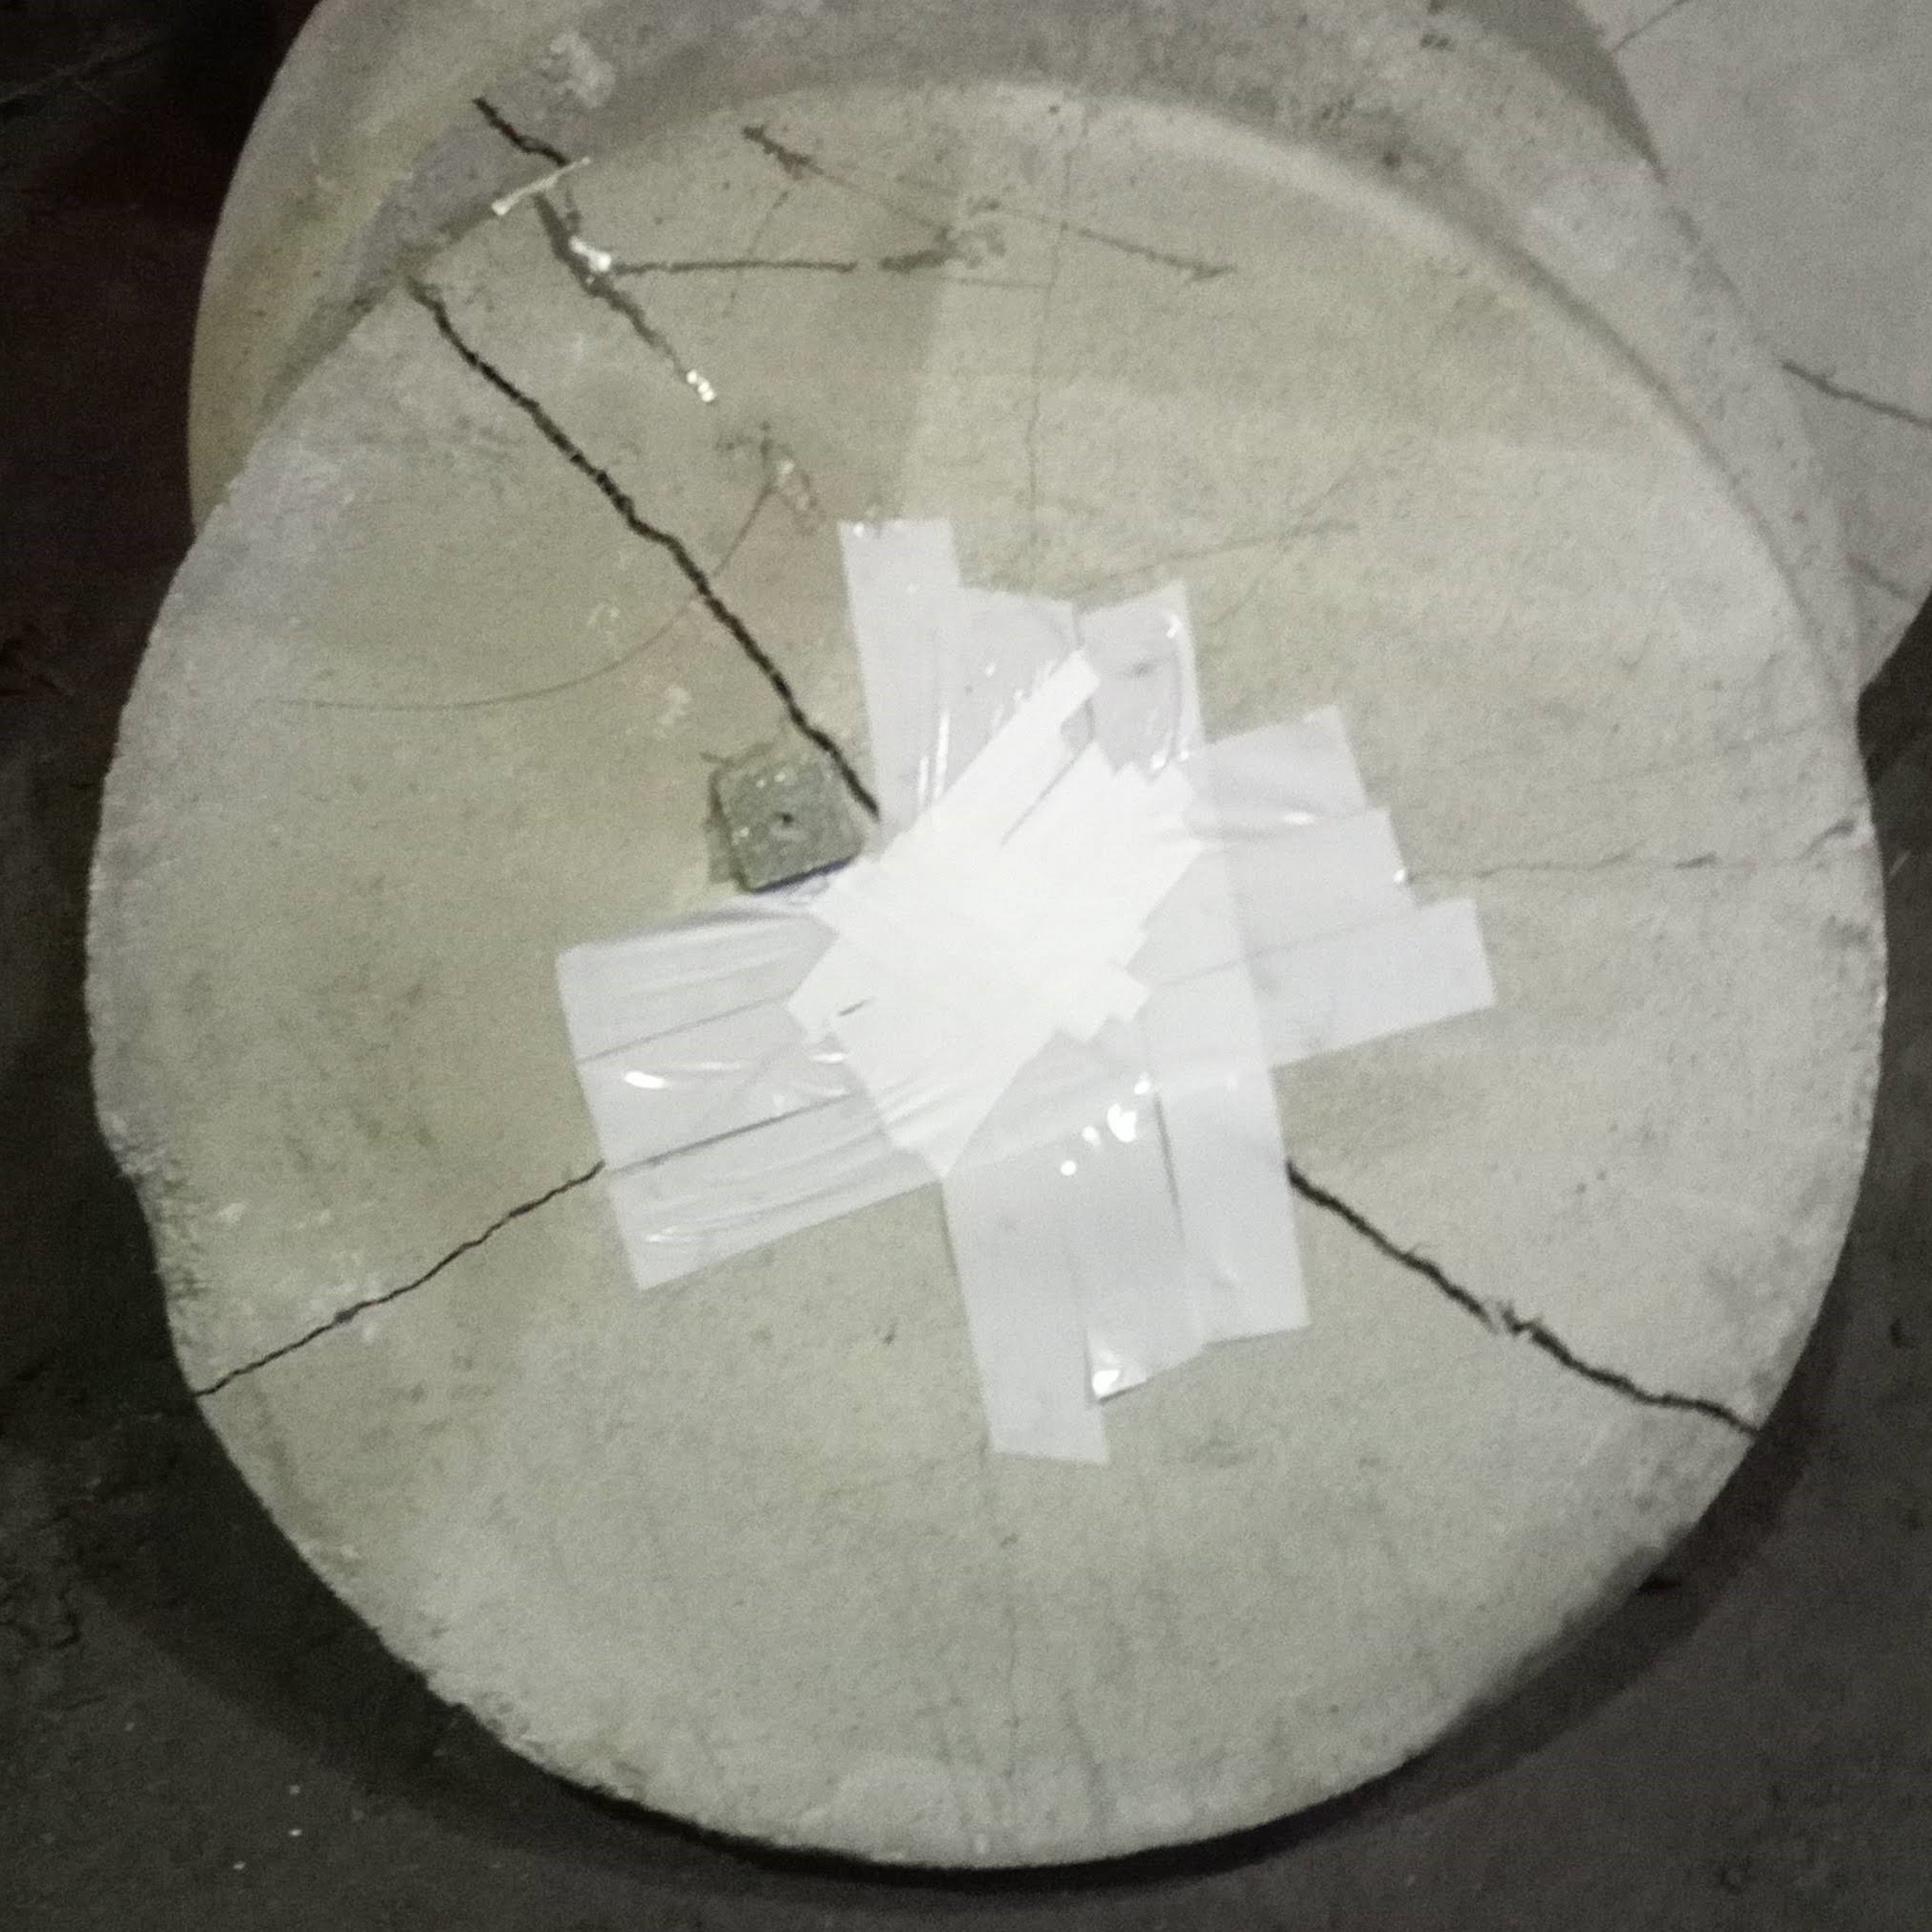
\includegraphics[width = 0.45\linewidth]{pics/basket.jpg}}

\caption{Different ways of applying tape to a sample}
\label{fig:beauty_tape}
\end{figure}

To contain the dust and create a smooth surface for the laser tape was glued on the samples. Two ways of gluing the tape on the concrete were tried.
Firstly the tape was applied in one layer in parallel strips. These were over stretched and ripped. See \autoref{fig:riptape}. Even though the tape ripped it reduced the development of dust significantly. 

Secondly the tape was applied in a basket weave pattern. With strips alternating vertically and horizontally crossing each other. See \autoref{fig:tape}.
This setup did not rip but it was prone to detaching from the sample.

If the displacement were to be measured using computer vision or photogrammetry in the future, covering the entire surface of the sample with a thin film of latex of another flexible stabiliser might reduce the dust production enough to yield usable results. For this thesis using photogrammetry to measure the displacement was considered but as the cameras would have to be placed above the sample and the expected deformations on top and on bottom are not the same this idea was discarded.


The high speed camera was the redundant sensor for measuring the deformation of the sample and it suffered a few failures as well.

\subsection{Increasing the Reliability of the High Speed Camera}

The failures of the high speed camera were all caused by operator mistakes. A check list was implemented to keep such errors from happening.

Even though the sensors malfunctioned at times enough data could be collected to get results.

\section{Results of Round Sample Tests}

The round samples were the first to be tested. The additional accelerometers attached directly to the sample yielded interesting insights into the way the impact propagated through the sample.

\subsection{Additional Accelerometer}

In \autoref{tab:acc_compare} the acceleration measured on the drop weight and on the sample are compared. The acceleration measured on the sample 2019-04-16\_Rfrs\_75\_0,5 is significantly higher because the impact velocity was much higher.

The drop weight appears to undergo overwhelmingly positive acceleration while the sample experiences both positive and negative acceleration. This is not surprising as the drop weight is already accelerated to the impact velocity before impact and has to decelerate down to zero. The sample is first accelerated downward and outward and deforming elastically before returning to its plastic post deformation shape.  The acceleration measured on the sample appears to be mostly biased towards positive acceleration. 

\begin{table}
    \centering
    \begin{tabular}{lllllll}
    \toprule
    Sample number		&   \multicolumn{2}{l}{Drop weight}	& \multicolumn{4}{c}{Sample} \\
    \cmidrule{4 - 7}
    			&		&							& \multicolumn{2}{l}{Vertical}	& \multicolumn{2}{l}{Horizontal}    \\
    \midrule
    5  & 1718,23 & - 120,42 & 3384,14 & - 2027,52 & &\\
    15 & 1389,15 & - 55,74 & 4919,99 & - 3825,53 & &\\
    16 & 3963,18 & - 931,50 & 1507,00 & -964,91 & 525,13 & - 564,48\\
    %\multicolumn{2}{c}{Drop weight} &   \multicolumn{2}{c}{Vertical}    &   \multicolumn{2}{c}{Horizontal}\\
    %\midrule
    %3963.18 & - 931.50 & 1507,00 & -964,91 & 525,13 & - 564,48\\
    \bottomrule
    \end{tabular}
    \caption{Comparing the acceleration [$\frac{\text{m}}{\text{s}^2}$] measured on drop weight to the acceleration measured directly on the sample}
    \label{tab:acc_compare}
\end{table}


\begin{figure} 
\centering 
\subcaptionbox{Bouncing as measured by the accelerometer \label{fig:accelBounce}}
{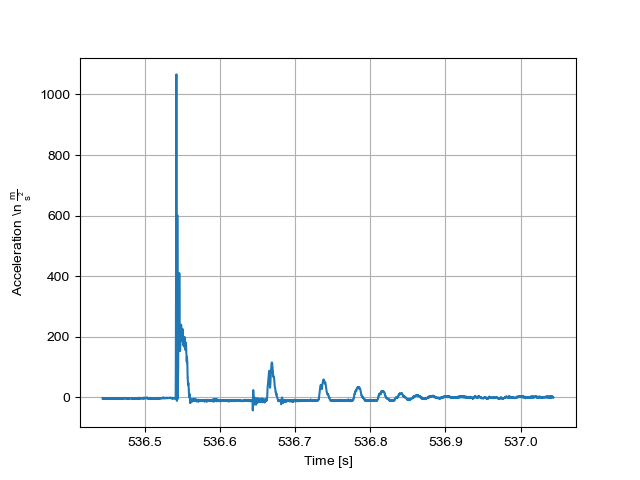
\includegraphics[width=0.45\linewidth]{pics/accelbounce.png}} 
\subcaptionbox{Bouncing as measured by the load cell \label{fig:loadBounce}} 
{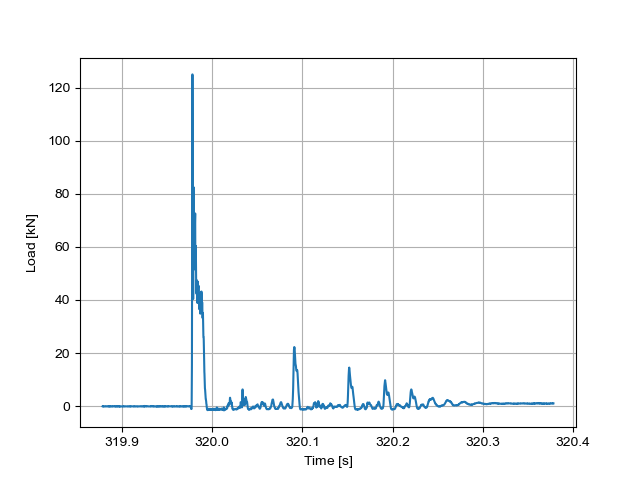
\includegraphics[width=0.45\linewidth]{pics/loadbounce.png}}

\caption{Bouncing of the drop weight after impact}
\label{fig:Bounce} 
\end{figure}

The additional accelerometers yielded interesting data about the behaviour of the sample. The drop weight seems to be reverberating for quite some time (200 ms), while the sample quickly settles in its new shape (2 ms). The accelerometer on the sample registers larger accelerations than the the sensor on the drop weight as displayed in \autoref{fig:acccom}. Note that 2019-02-20\_Rfrs\_100\_1,0 broke during testing  and 2019-04-16\_Rfrs\_75\_0,5 only cracked. This explains the longer vibration time of 2019-02-20\_Rfrs\_100\_1,0. From this graphic it is obvious that the vertical acceleration and the horizontal acceleration both look similar to each other.

\begin{figure}
    \centering
    \subcaptionbox{Step 0: Before impact \label{fig:bounce0}}
    {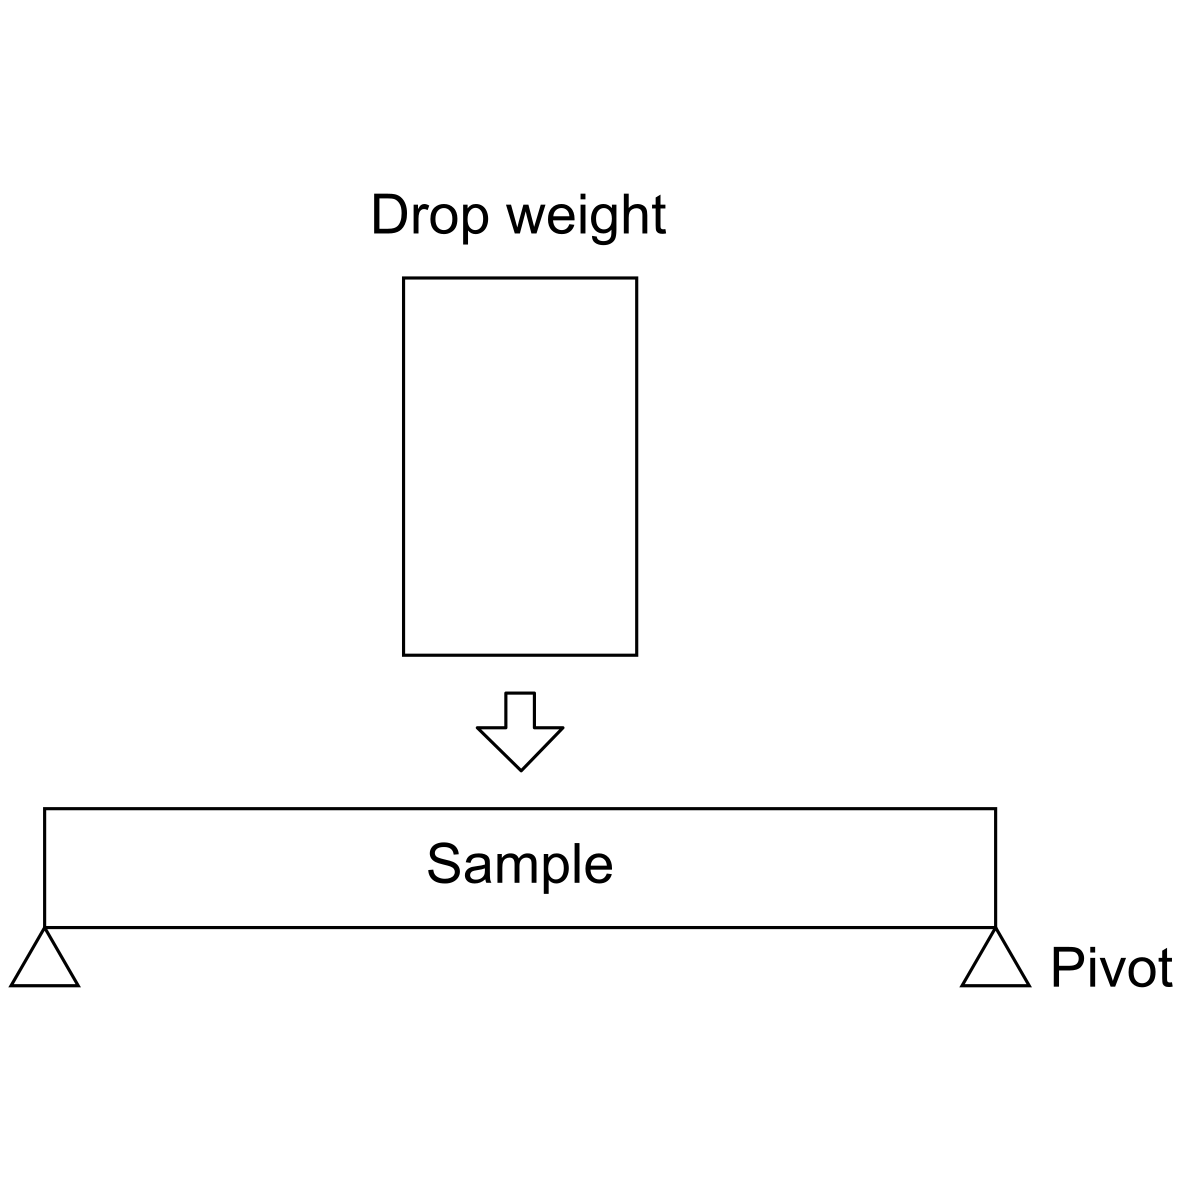
\includegraphics[width = 0.45\linewidth]{pics/bounce_0.png}}
    \subcaptionbox{Step 1: Sample deforms plastic and elastic \label{fig:bounce1}}
    {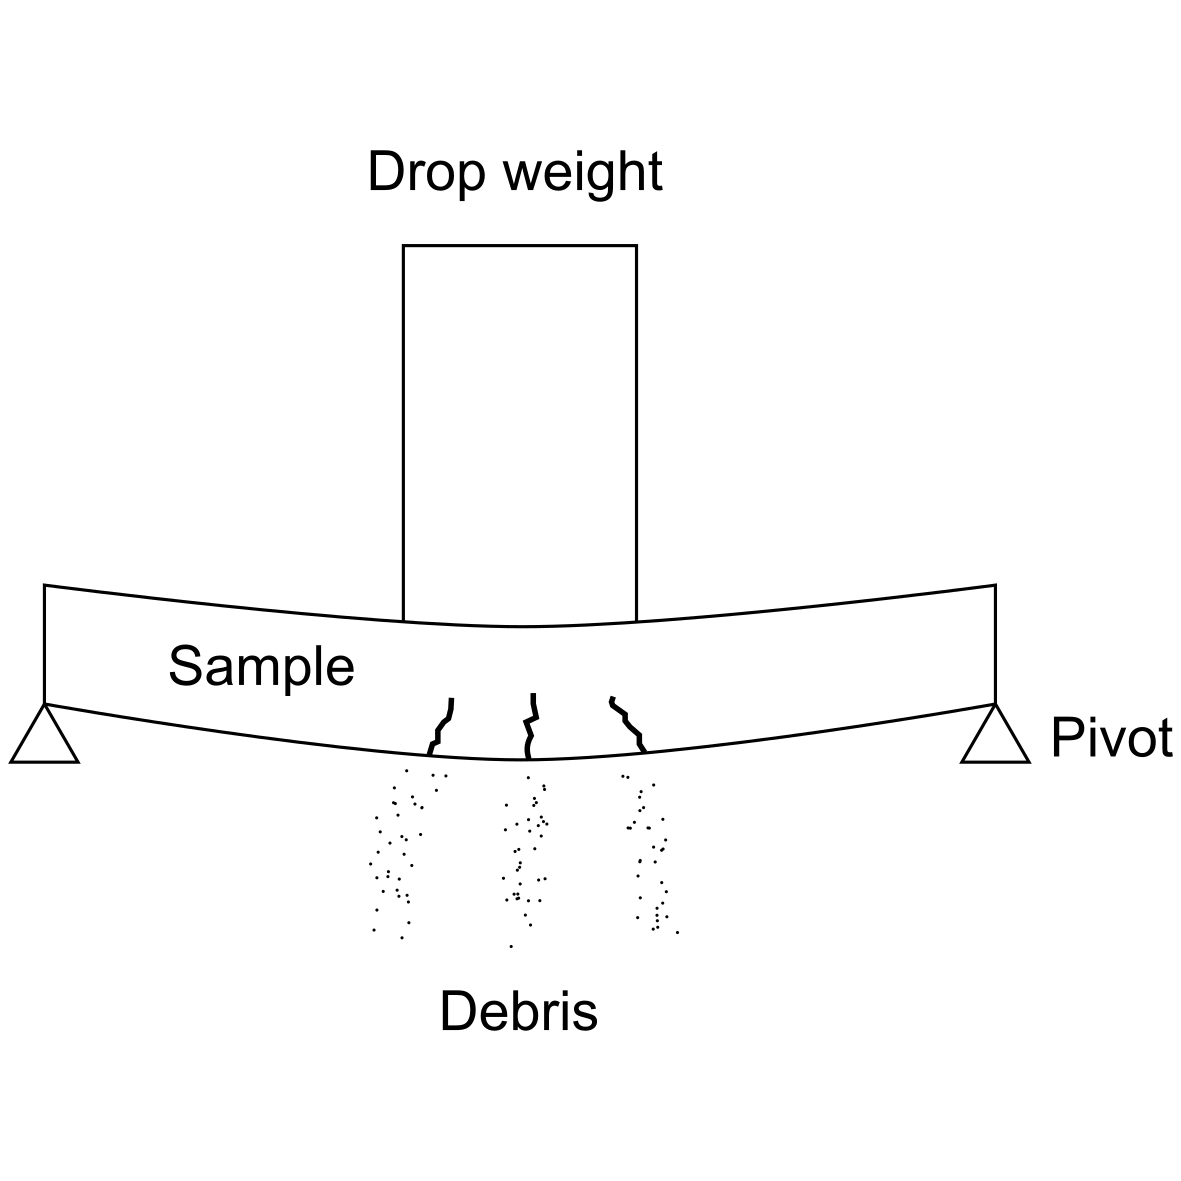
\includegraphics[width = 0.45\linewidth]{pics/bounce_1.png}}
    
    \subcaptionbox{Step 2: Elastic deformation energy is \\ released, sample and drop weight jump \label{fig:bounce2}}
    {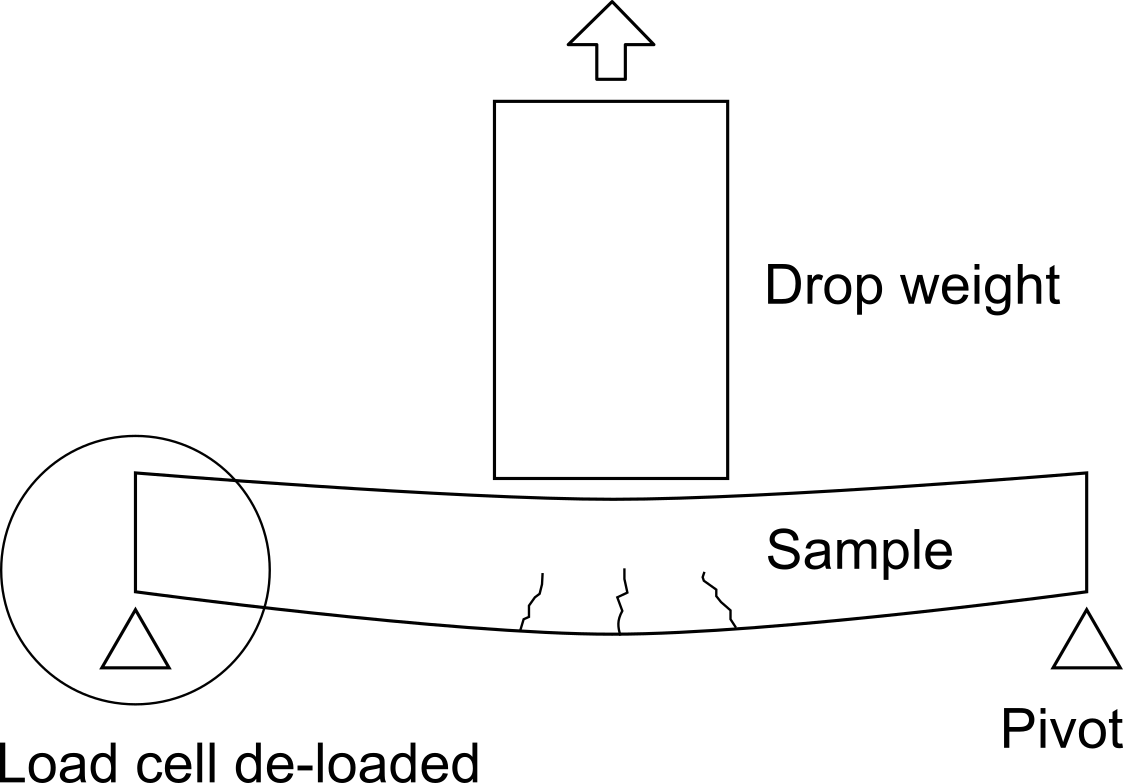
\includegraphics[width = 0.45\linewidth]{pics/bounce_2.png}}
    \subcaptionbox{Step 3: Sample and drop weight drop again \label{fig:bounce3}}
    {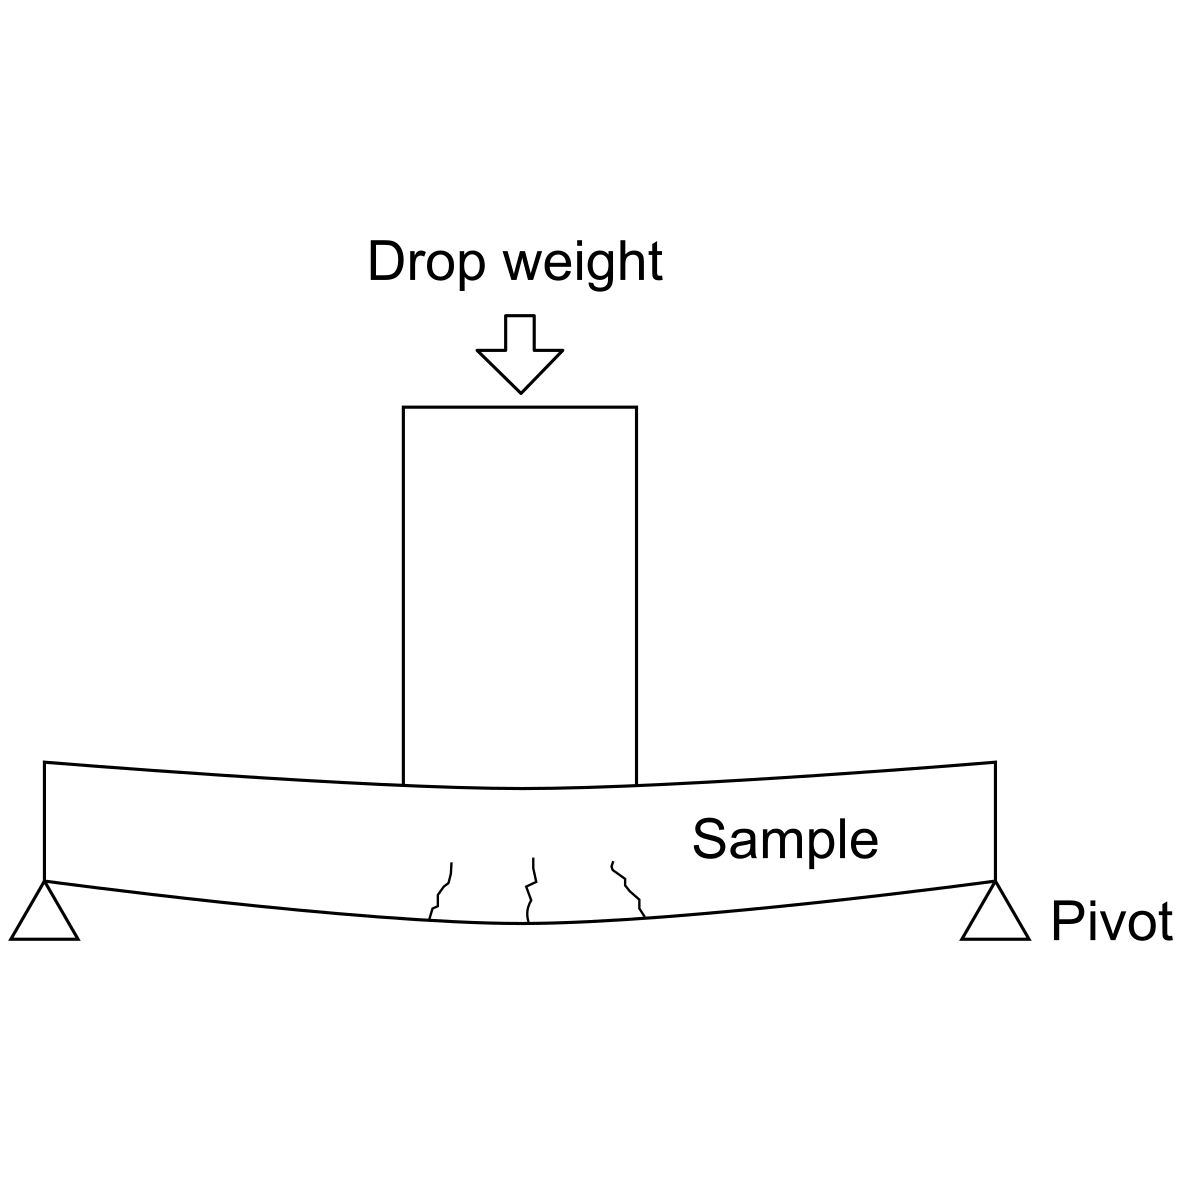
\includegraphics[width = 0.45\linewidth]{pics/bounce_3.png}}
    \caption{The mechanism behind the bouncing of the sample}
    \label{fig:bounce}
\end{figure}

In the high speed footage taken of sample 2019-08-19\_Rfrs+t\_75\_1,0 it appears that the entire sample jumps upwards a few millimeters following the initial impact. The bouncing appears to follow a simple pattern. See \autoref{fig:bounce}.

In \autoref{fig:bounce1} the initial impact is displayed the sample cracks and debris is expelled from the cracks. The sample experiences maximum deformations at this point and the  vast majority of the cracks is formed. 

The elastic deformation energy is released again after the initial impact and both sample and drop weight bounce upwards and either complete de-load the load cells or at least reduce the load on them. The drop weight jumps slightly higher than the sample. In the high speed camera footage it looks as if the sample has already settled into its new position when it is struck by the second impact. 
See \autoref{fig:bounce2}.

Sample and drop weight fall back down. The sample experiences more elastic and plastic deformation. This is displayed in \autoref{fig:bounce3}.

Step 2 and 3 repeat until the entire impact energy has been dissipated.

Some discord exists between readings of the additional accelerometers and the high speed camera. The accelerometers show that the acceleration of the sample stabilizes very quickly (2 ms) while it is bouncing for a significant amount of time (400 ms) on the high speed camera footage. No test with good high speed camera coverage and additional accelerometers exists. This makes this phenomenon even harder to explain.

Initially it was supposed that the accelerometer on the sample could be used to calculate the displacement. The measurements showed a lot of zero drift an zero offset after integrating them to get the impact velocity and the displacement. These errors had to be removed in post processing. As no sample has working additional accelerometers and displacement measurements it was not possible to calibrate the double integrated curves. They were deemed to unreliable to use in this analysis.

\begin{figure}
    \centering
\subcaptionbox
{Acceleration measured on drop weight for 2019-02-20\_Rfrs\_100\_1,0
\label{fig:accdropweight1}}
{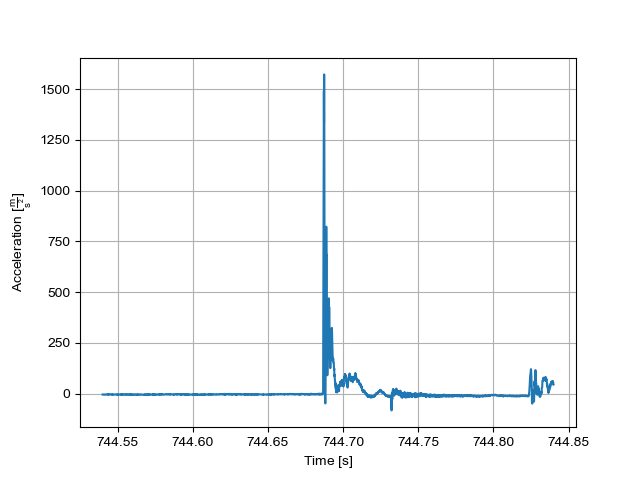
\includegraphics[width = 0.45\linewidth]{graph/2019-02-20_Rfrs_100_1,0.png}}
\subcaptionbox
{Vertical acceleration measured on sample for 2019-02-20\_Rfrs\_100\_1,0
\label{fig:accvertical1}}
{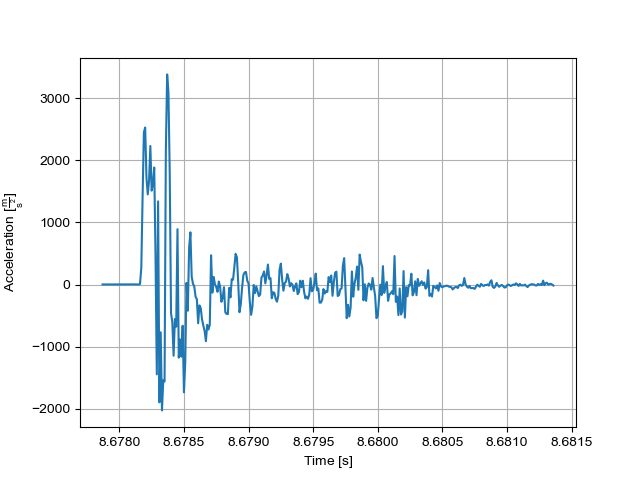
\includegraphics[width = 0.45\linewidth]{graph/2019-02-20_Rfrs_100_1,0_vertical.png}}

%\subcaptionbox
%{Acceleration measured on drop weight for 2019-02-20\_Rfrs\_100\_0,5
%\label{fig:accdropweight2}}
%{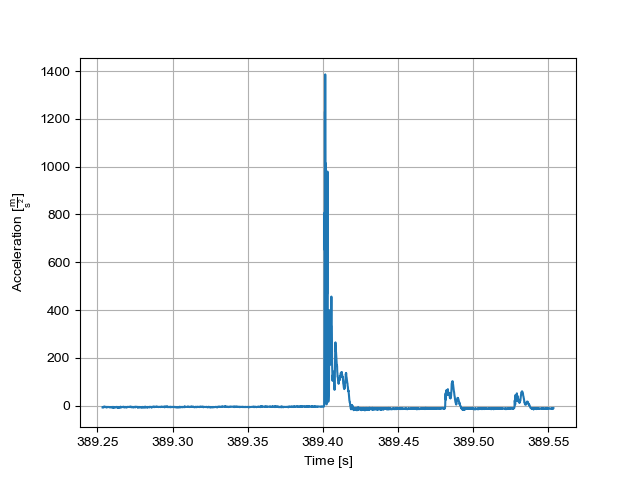
\includegraphics[width = 0.45\linewidth]{graph/2019-02-20_Rfrs_100_0,5.png}}
%\subcaptionbox
%{Vertical acceleration measured on drop sample for 2019-02-20\_Rfrs\_100\_0,5
%\label{fig:accvertical2}}
%{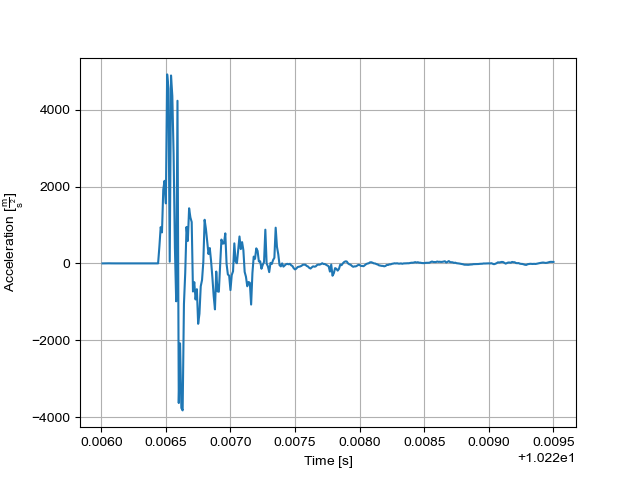
\includegraphics[width = 0.45\linewidth]{graph/2019-02-20_Rfrs_100_0,5_vertical.png}}

\subcaptionbox{Acceleration measured on drop weight for 2019-04-16\_Rfrs\_75\_0,5} {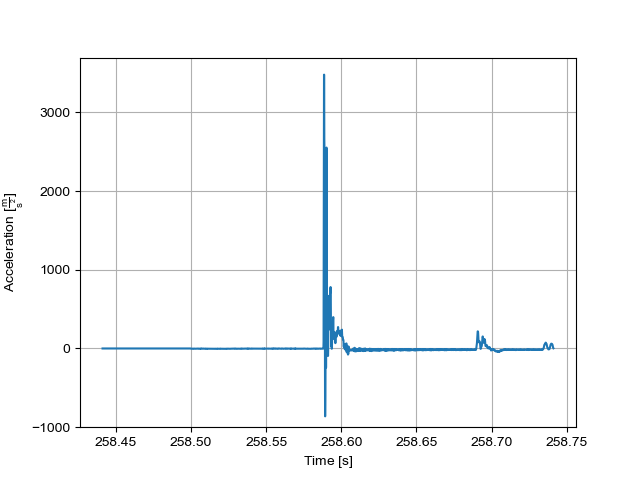
\includegraphics[width=0.45\linewidth]{graph/2019-04-16_Rfrs_75_0,5.png}}
    
\subcaptionbox{Vertical acceleration measured on drop sample for 2019-04-16\_Rfrs\_75\_0,5  }{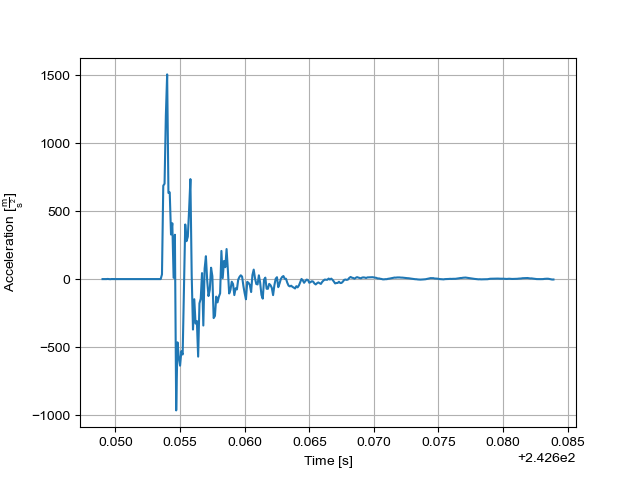
\includegraphics[width=0.45\linewidth]{graph/2019-04-16_Rfrs_75_0,5_vertical.png}}
\subcaptionbox{Horizontal acceleration measured on drop sample for 2019-04-16\_Rfrs\_75\_0,5
}{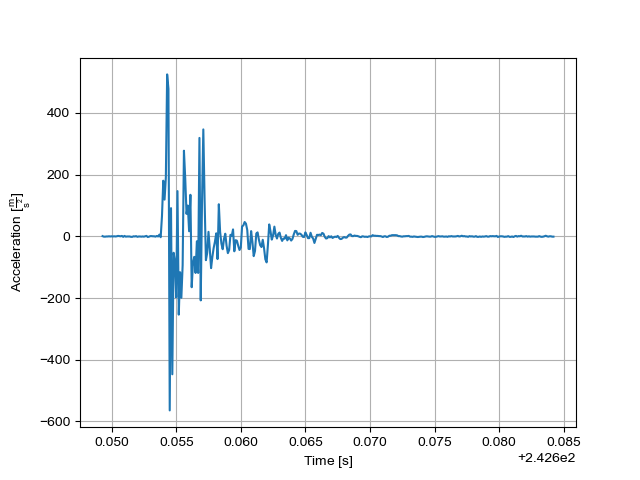
\includegraphics[width=0.45\linewidth]{graph/2019-04-16_Rfrs_75_0,5_horizontal.png}}

\caption{Comparing the measured acceleration on drop weight and on sample}
\label{fig:acccom}
\end{figure}

\begin{figure}
    \centering
    \subcaptionbox{sample 2019-02-20\_Rfs\_75\_0,5}{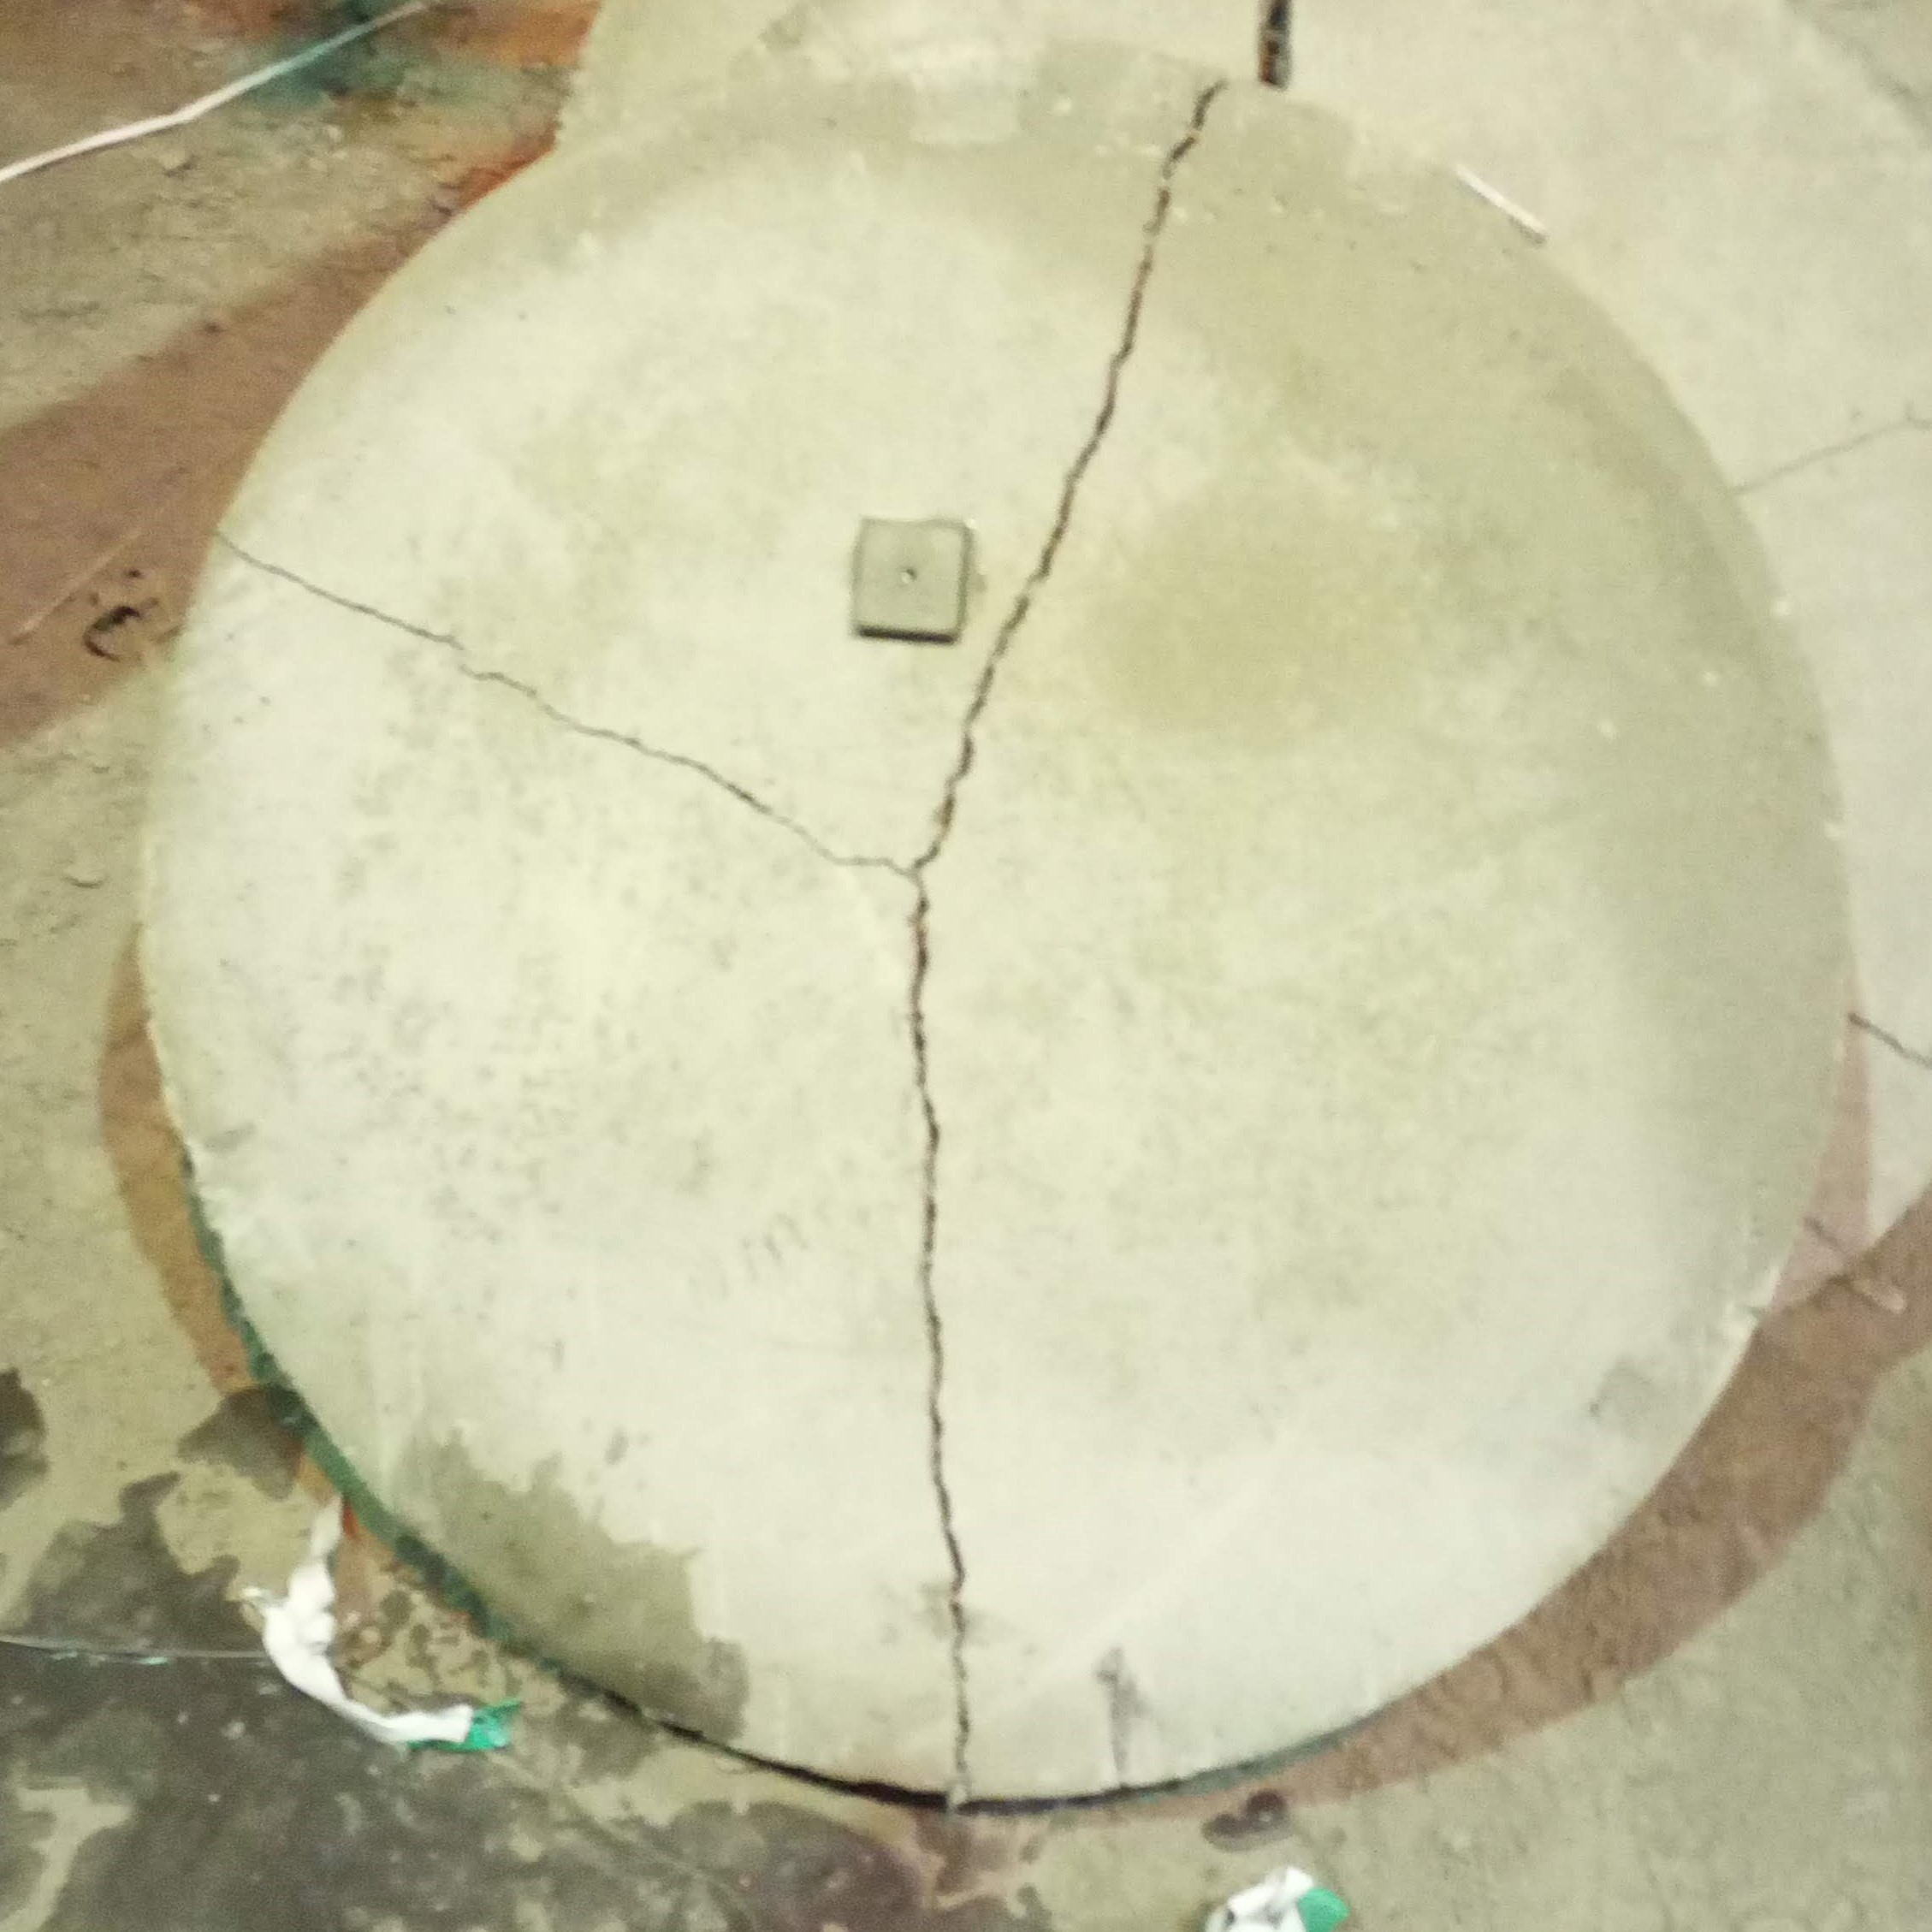
\includegraphics[width = 0.45\linewidth]{appendix/2019-02-20_Rfrs_75_0,5.jpg}}
    \subcaptionbox{sample 2019-04-16\_Rfrs\_75\_0,5}{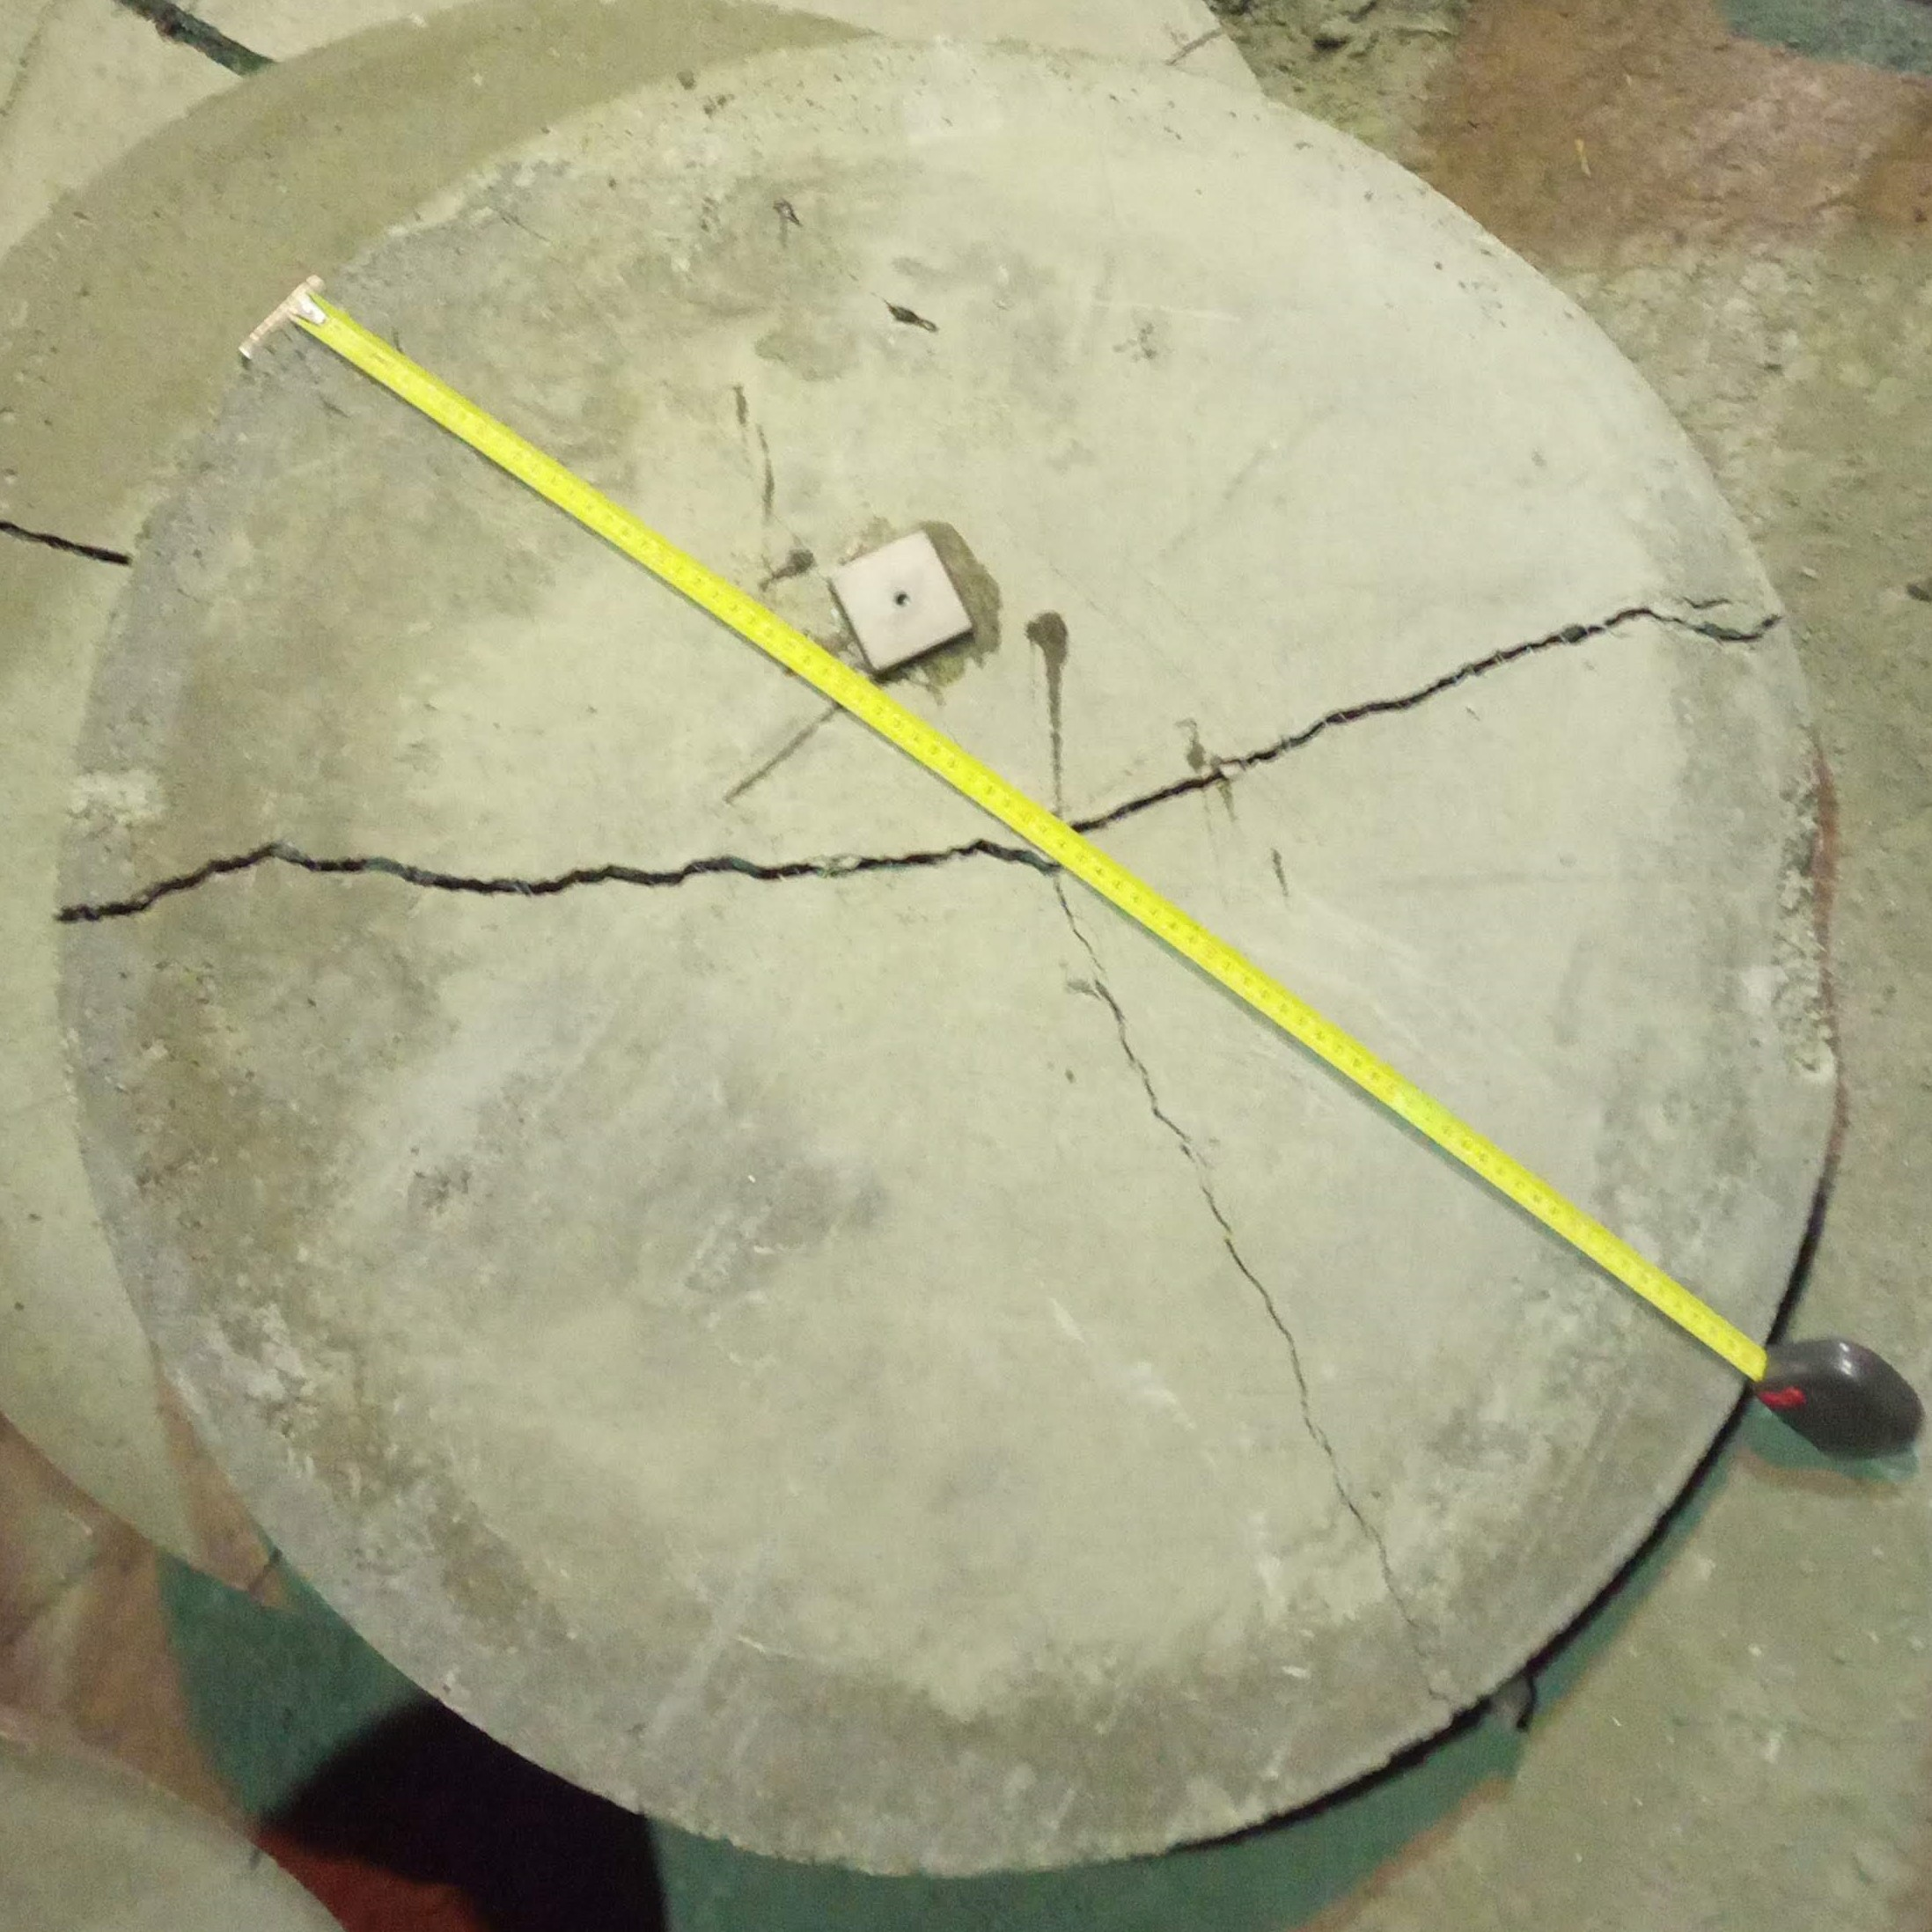
\includegraphics[width = 0.45\linewidth]{appendix/2019-04-16_Rfrs_75_0,5.jpg}}

    \subcaptionbox{sample 2019-05-06\_Rfrs\_75\_0,8}{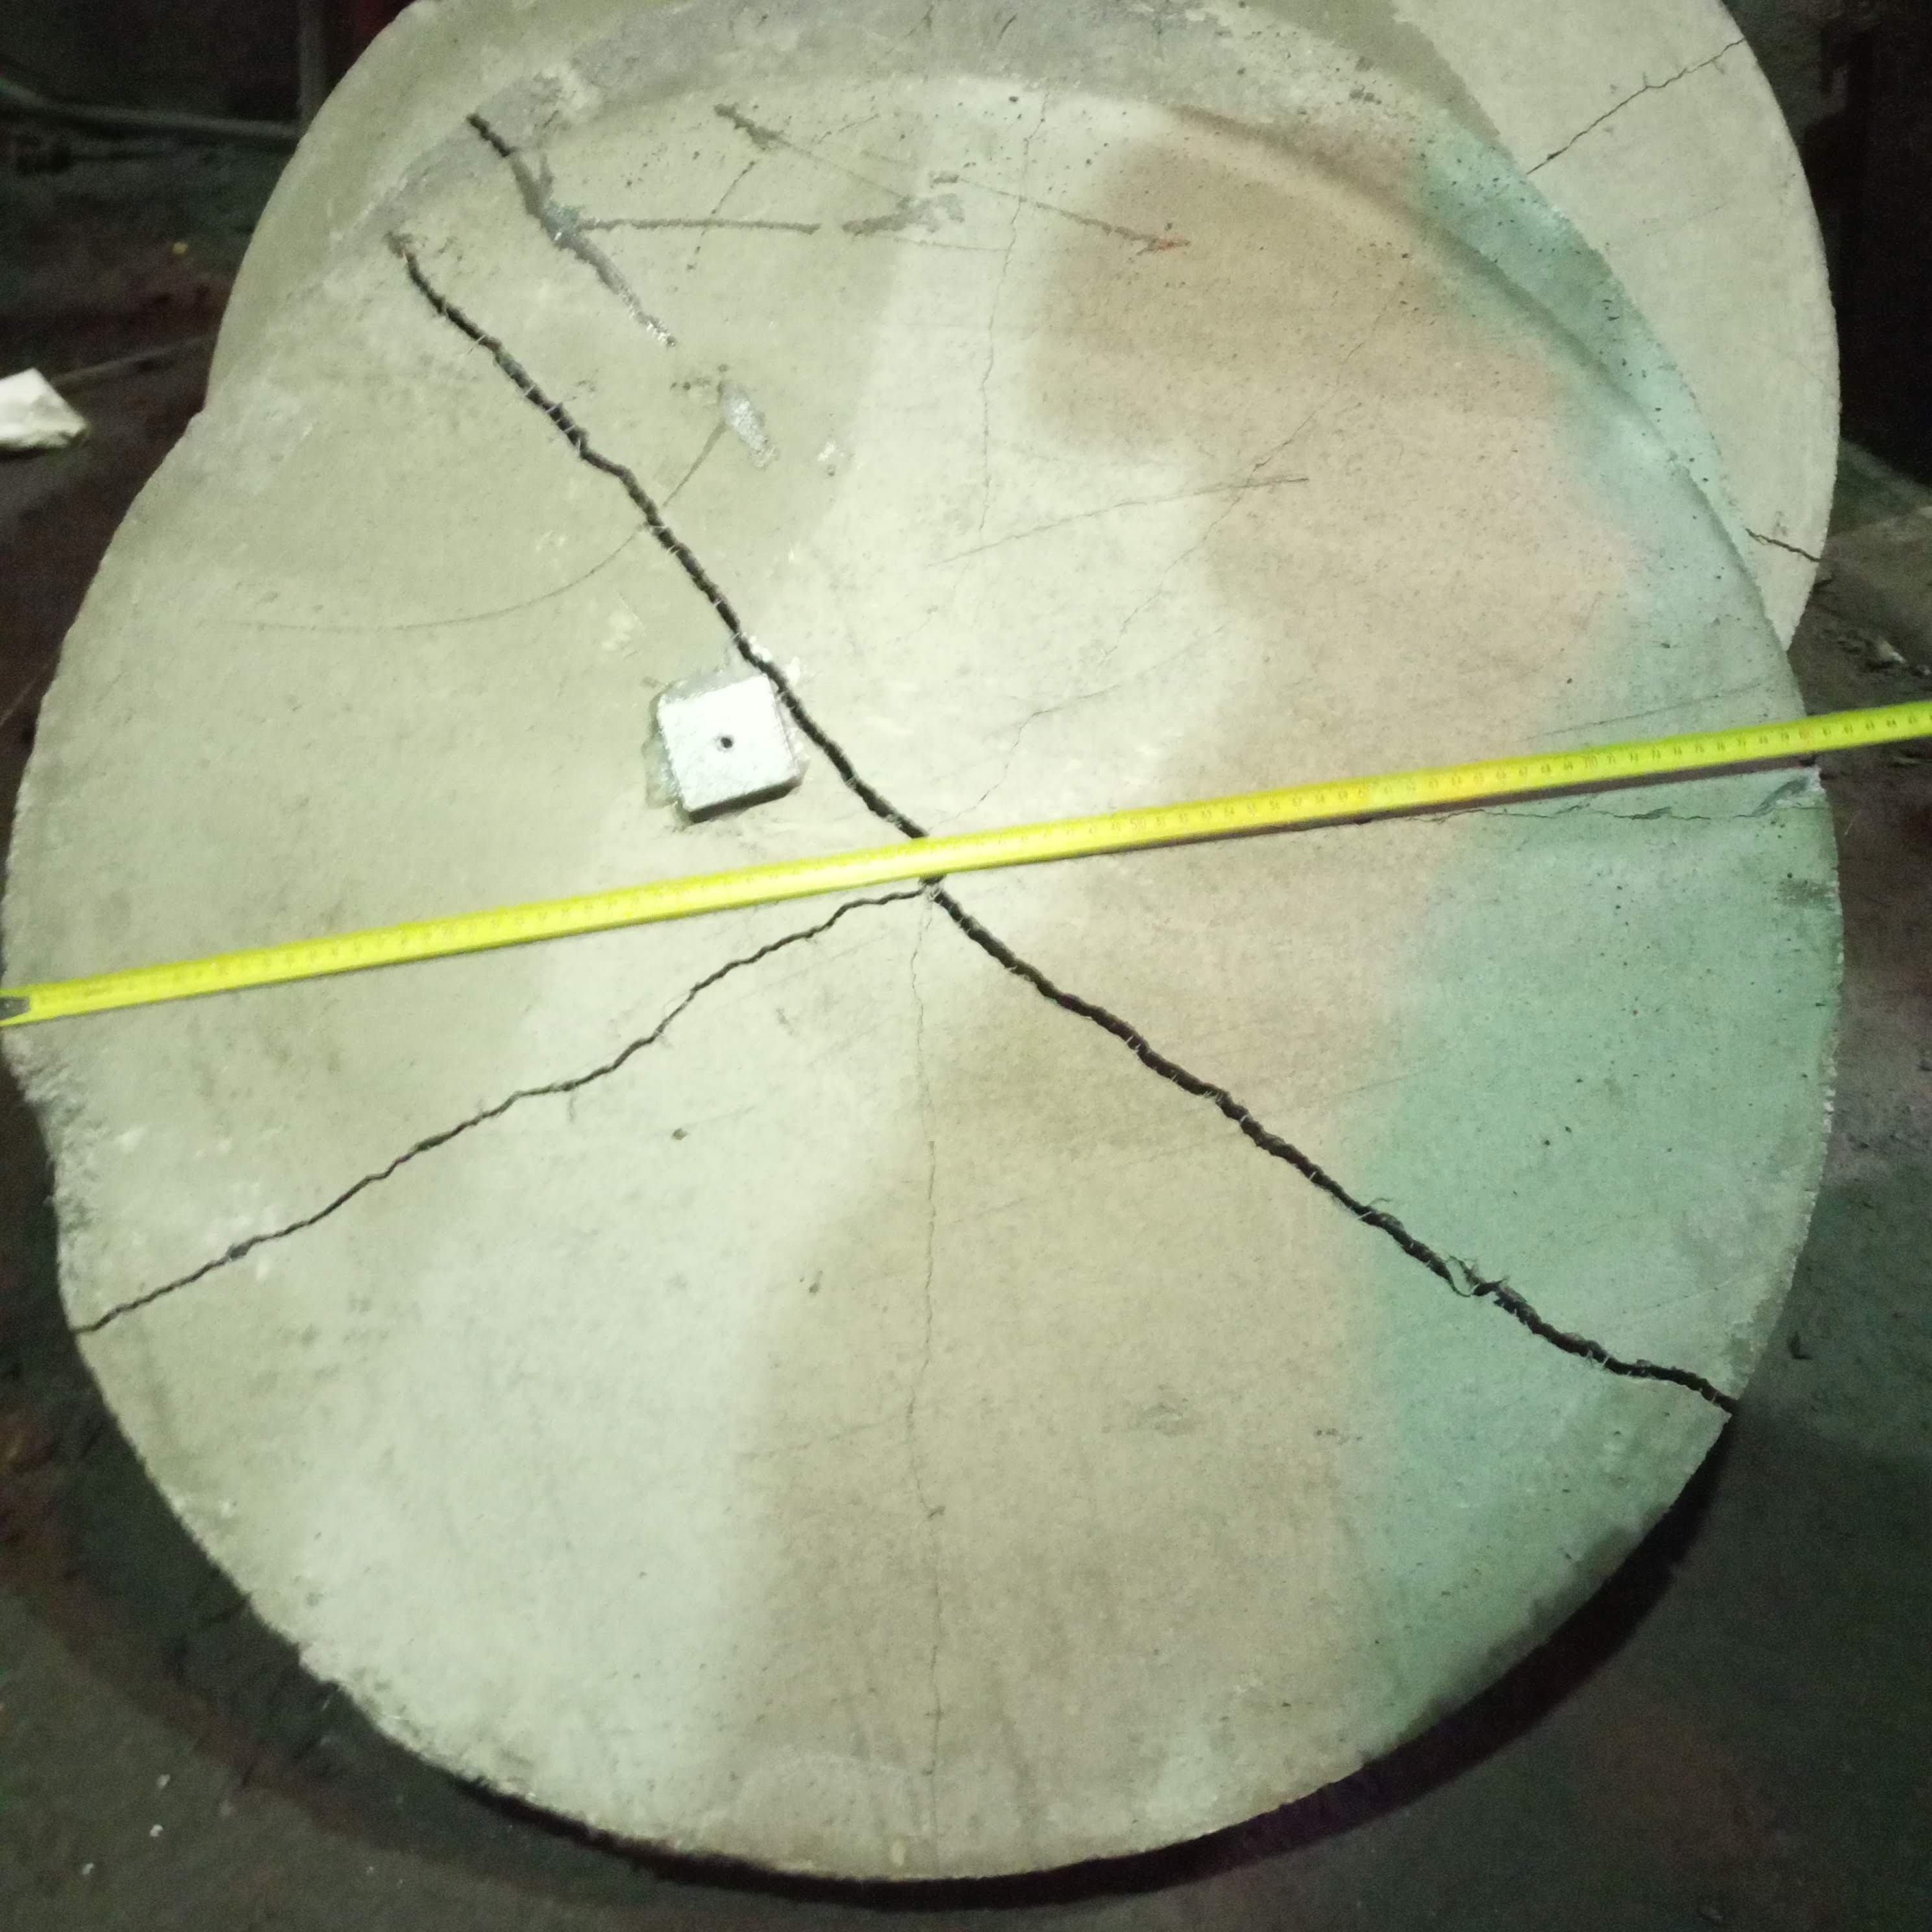
\includegraphics[width = 0.45 \linewidth]{appendix/2019-05-06_Rfrs_75_0,8.jpg}}
    \caption{Crack pattern of samples with additional accelerometers}
    \label{fig:crack_accel}
\end{figure}

\begin{figure}
    \centering
    \begin{tikzpicture}
%sensor array of second campaign under view


%sample
\draw(4,4) circle [radius=4];

%load cells
\draw [fill = blue] (90:3.75) ++ (4,4) circle [radius=.25]
 (210:3.75) ++ (4,4) circle [radius=.25]
 (-30:3.75) ++ (4,4) circle [radius=.25];
\draw (-30:5) ++ (4,4) node (load) {load cell}
(3,6) node [align=center] {expected cracks};

%accelerometers
\draw (4,4) ++ (210:1.5) coordinate (accel);
\draw[rotate=120] (accel) -| ++ (0.25,-0.5) coordinate [pos=0] (that)  -| ++ (-0.5,0.5)  -- cycle;
\draw[fill = red] (4,4) ++ (210:1.25) circle [radius=.1];
\path (4,4) -- ++ (-110:4) coordinate (side);
\draw[rotate=-20] (side) -| ++ (0.25,-.1)  -|  ++ (-0.5,0.1) -- cycle;
\draw[rotate=-20, fill=red] (side) ++ (0.1,-0.1) -- ++ (0,-.2) arc (0:-180:0.1) coordinate [pos=0.7] (here) -- ++ (0,.2);
\draw (0,-1) node (this) {accelerometer};
\draw [-{Latex[length=3mm, width=1mm]}] (this) -- (that);
\draw [-{Latex[length=3mm, width=1mm]}] (this) -- (here);

%cracks
%\path[clip] (4,4) -- ++ (25:4) arc (25:35:4) -- 
%(4,4) -- ++ (145:4) arc (145:155:4) -- 
%(4,4) -- ++ (265:4) arc (265:275:4) -- cycle;

%\path[clip] (4,4) -| ++ (0.2,-5) -| ++ (-0.4,5) -- (4,4) -- ++ (-60:0.2) -- ++ (30:5) -- ++ (120:0.4) -- ++ (-150:5) -- (4,4) -- ++ (60:0.2) -- ++ (150:5) -- ++ (240:0.4) -- ++ (330:5) --cycle;

%\path[fill = lightgray] (4,4) circle [radius = 0.23];
\begin{scope}


\path[clip] (4,4) -| ++ (0.2,-5) -| ++ (-0.4,5) -- cycle
(4,4) -- ++ (-60:0.2) -- ++ (30:5) -- ++ (120:0.4) -- ++ (-150:5) -- cycle 
(4,4) -- ++ (60:0.2) -- ++ (150:5) -- ++ (240:0.4) -- ++ (330:5) --cycle;


\draw [fill=lightgray] (4,4) circle [radius=4];
\end{scope}
\draw[fill=red] (3.5,3.5) rectangle (4.5,4.5);
\draw
(4,5) node {tape};

\end{tikzpicture}
    \caption{Expect crack pattern relative to position of additional accelerometers and loadcells}
    \label{fig:senunder}
\end{figure}

It is possible that the metal plates for the additional accelerometers affected the formation of cracks. When studying \autoref{fig:crack_accel} it becomes obvious that there is one large crack almost straight through the sample. In two cases it went between the two accelerometers. This failure mode was not expected. The samples were supposed to have 3 similarly large cracks with the accelerometer approximately in the middle between two of them, see \autoref{fig:senunder}, the expected failure pattern is shaded in gray. These areas are the ones under tension when the panel is loaded and \autocite{c1550} describes this as the typical failure pattern. 

It was also observed that the samples with additional accelerometers broke at lower energy levels. There are 11 samples with a thickness of 75 mm. Additional accelerometers were used on 5 of them. Without additional accelerometers no sample broke below a 1 kJ impact. The highest impact survived by a sample with additional accelerometers was 0,74 kJ, two samples broke at 1 kJ. Together with the marked change in crack pattern the accelerometers appear to weaken the samples.


\subsection{Load - Displacement Curves}

\begin{figure}
    \centering
    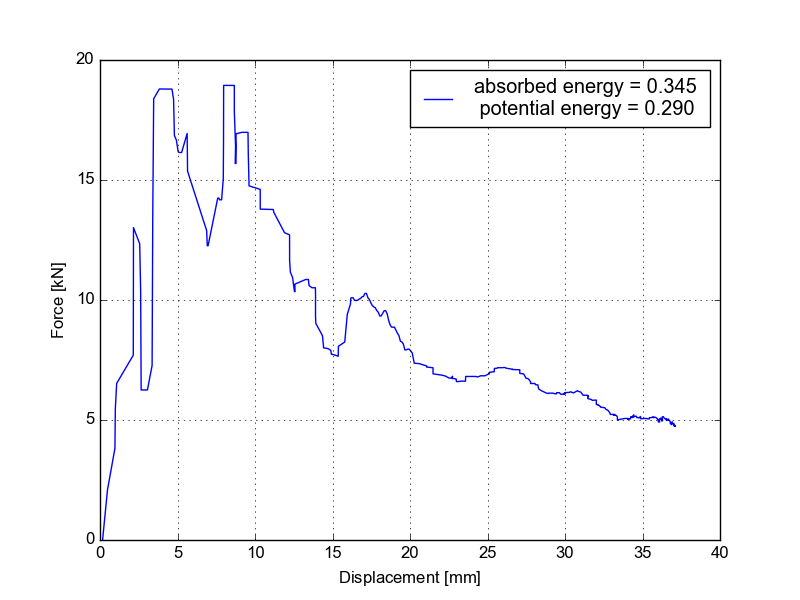
\includegraphics[width=0.95 \linewidth]{pics/2018-12-04_Rfrs_50_0,3_2_energy.png}
    \caption{Energy absorbed during test 2018-12-04\_Rfrs\_50\_0,3\_2}
    \label{fig:energy1}
\end{figure}

\begin{figure}
    \centering
    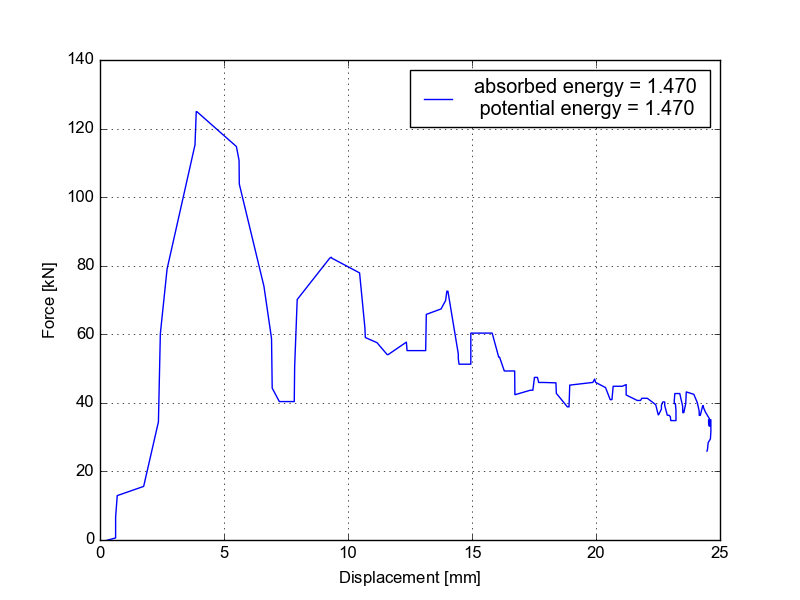
\includegraphics[width=0.95 \linewidth]{pics/2018-12-10_Rfrs_100_1,5_energy.png}
    \caption{Energy absorbed during test 2018-12-10\_Rfrs\_100\_1,5}
    \label{fig:energy2}
\end{figure}

\begin{figure}
    \centering
    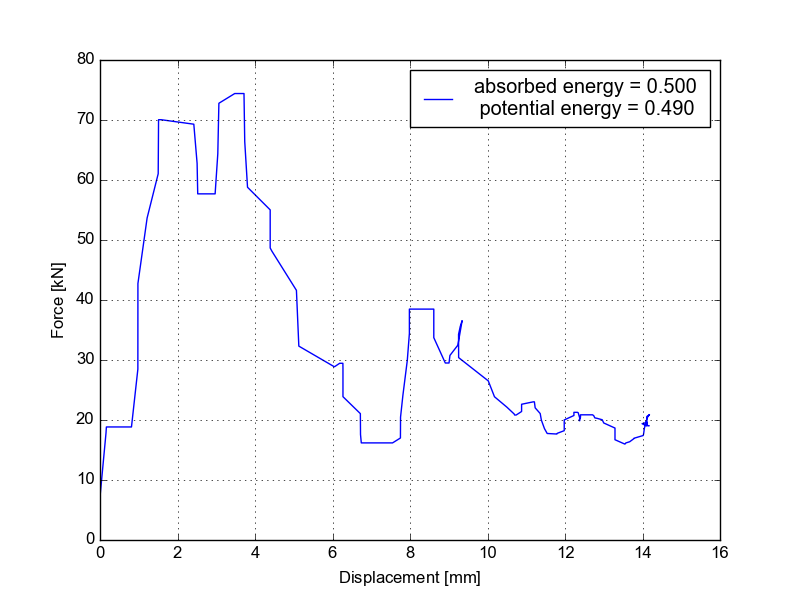
\includegraphics[width = 0.95\linewidth]{pics/2019-02-20_Rfrs_75_0,5_energy.png}
    \caption{Energy absorbed during test 2019-02-20\_Rfs\_100\_0,5}
    \label{fig:energy3}
\end{figure}

\begin{figure}
    \centering
    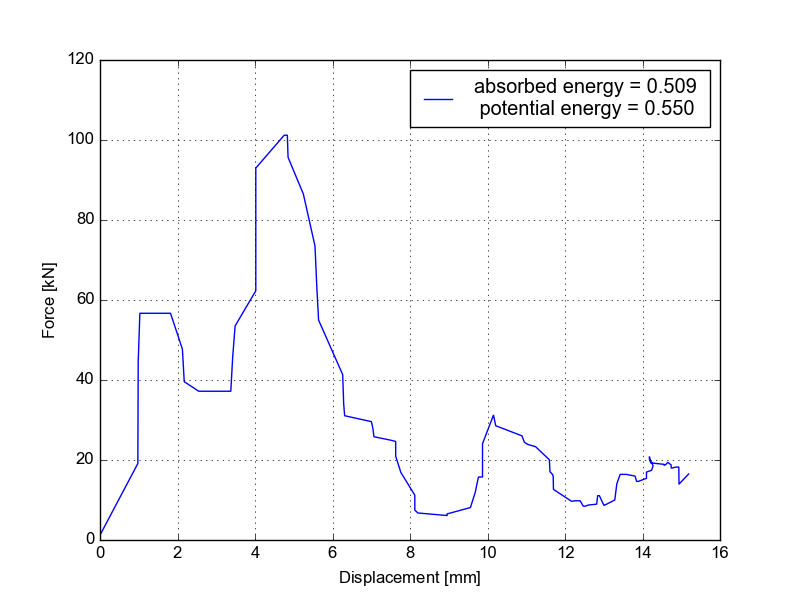
\includegraphics[width=0.95 \linewidth]{pics/2019-04-16_Rfrs_75_0,5_energy.png}
    \caption{Energy absorbed during test 2019-04-16\_Rfrs\_75\_0,5}
    \label{fig:energy4}
\end{figure}

\begin{figure}
    \centering
    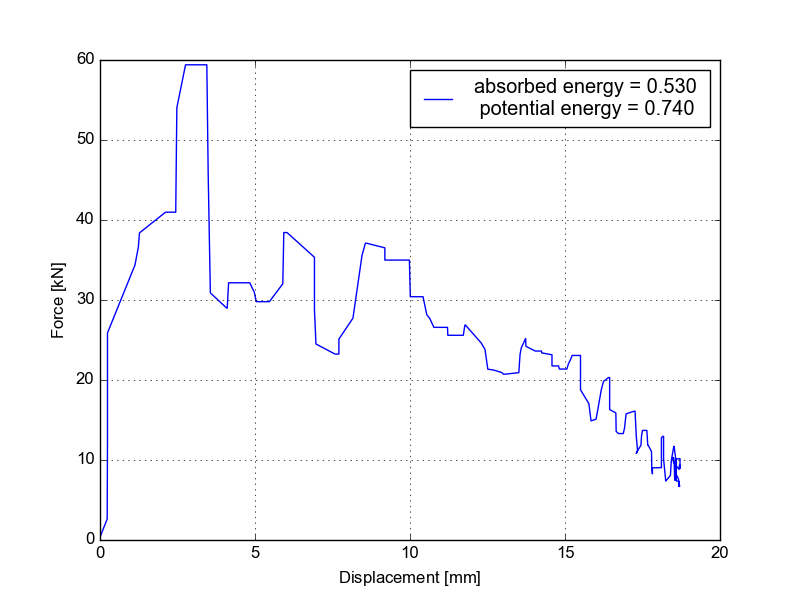
\includegraphics[width=0.95 \linewidth]{pics/2019-05-06_Rfrs_75_0,8_energy.png}
    \caption{Energy absorbed during test 2019-05-06\_Rfrs\_75\_0,8}
    \label{fig:energy5}
\end{figure}

The energy levels used in the analysis of the experiments are the calculated potential energy.
Of course it would be more accurate to calculated the absorbed energy through the load/displacement curve.
As the laser sensor readings were a bit erratic before the tape was applied drawing load/displacement curves and analysing the amount of absorbed energy is only possible for a few tests. 
See \autoref{fig:energy1}, \autoref{fig:energy2}, \autoref{fig:energy3}, \autoref{fig:energy4} and \autoref{fig:energy5}. 
The displacement measurement and the load measurements were synchronised to start at the same time. The initial dip in load was discarded to not interfere with the measurement. 
Some of the displacement curves were cleaned up significantly to be usable. 
The displacement has two parts: the elastic peak deformations and the plastic post peak deformations. 
The curves were drawn until the maximum deformation was reached. 
For two samples the energy absorbed that way was higher or equal to the the potential energy of the drop weight. 
This is of course impossible. 
Energy is dissipated through friction, bouncing, crushing and other factors. 
Therefore the energy measured by the load displacement curves should be lower than the potential energy. 
Some of the energy calculated from the load displacement curves would be released again if the curves had been drawn until the sample deformations had stabilised. 
For the sample 2018-12-04\_Rfrs\_50\_0,3\_2 the very large deformations led to a excessive large energy absorption capacity. It is not clear how the samples managed to derform so much.
For sample 2019-05-06\_Rfrs\_75\_0,8 a lot less energy was absorbed than the drop weight had. It is not clear what caused this discrepancy. There is a strong fluctuation in the displacement curve.
See appendix.
It is not easy to draw load displacement curves with the current sensor data and the energy derived from load displacement curves appears to be questionable at best.
When considering all load curves, see appendix, it is obvious that the thicker panels transfer the force much more quickly than the thinner panels

Overall it seems like using the potential energy to estimate the impact energy is good enough for the round panels. But how are the other parameters affected by the impact energy?



%%%%%%%%%%%%% LINEAR REGRESSION
\subsection{Linear Regression}
\label{ssec:linear}

The results of all tests are summarized in \autoref{tab:leg}. Each test is assigned a number to make them more easily accessible in the following figures. In the text samples will be referred to by (\textit{Number}) \textit{Name}. 
For example: (1) 2017-12-20\_Rfrs\_75\_1,8. The samples were numbered in the order they were tested in.
In \autoref{fig:heat} the coefficient of determination (\(R^2\)) of each parameter pair is displayed in a heat map. \(R^2\) is the normalized mean squared distance of each data point to the linear regression curve. \(R^2\) is a value between 1 and 0. \(R^2~=~1\) signifies perfect linear correlation, with all data points forming a perfect line.
\(R^2~=~0\) signifies a random distribution.
Values that correlate well are dark. Values that do not correlate are light.

\begin{figure}[h]
    \centering
    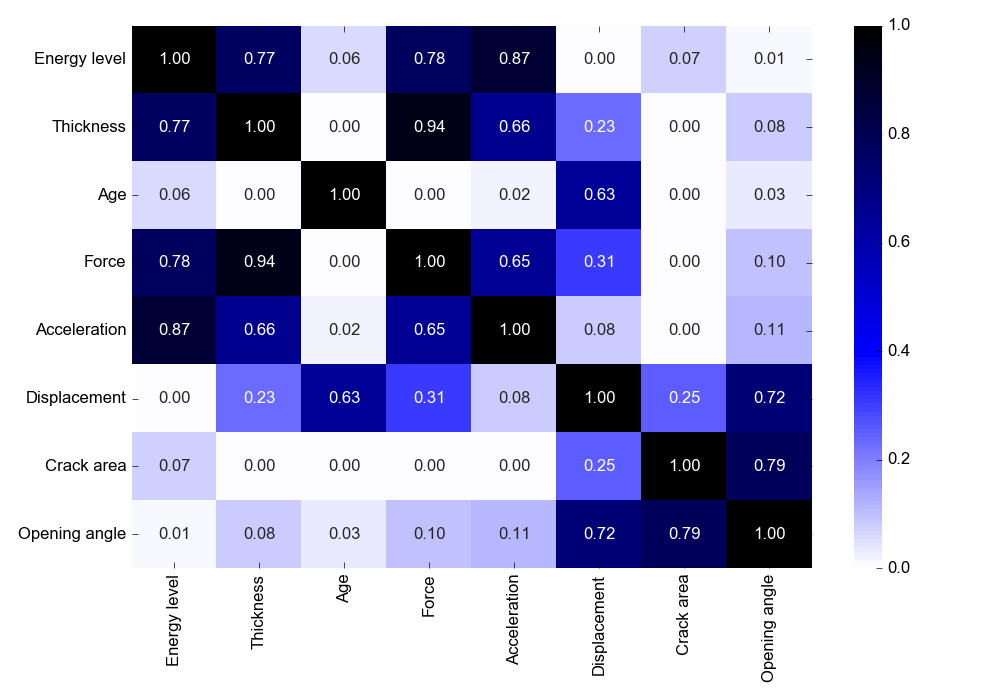
\includegraphics[width = 0.95\linewidth]{diagram/heatmap.png}
    \caption{Heat map of the correlation of various parameters}
    \label{fig:heat}
\end{figure}

\begin{landscape}
\begin{table}
    \centering
\begin{tabular}{l l l l l l l}
\toprule
Name & Number &   Force & Acceleration & Displacement & Crack area & Opening angle \\
&        &         &              &              &            &               \\
\midrule
2017-12-20\_Rfrs\_75\_1,8       &      1 &    3.24 &       278.03 &         -376 &            &               \\
2017-12-20\_Rfrs\_75\_3,5       &      2 &    2.22 &       765.97 &       -168.7 &            &               \\
2018-02-14\_Rfrs\_75\_1,0       &      3 &   75.32 &      1550.01 &         -0.3 &     25.000 &          17.1 \\
2018-02-14\_Rfrs\_75\_0,5       &      4 &   81.38 &      1119.83 &         -0.3 &      4.200 &           1.9 \\
2018-11-09\_Rfrs\_75\_0,5       &      5 &   60.56 &       504.77 &          0.1 &     16.400 &           9.1 \\
2018-11-29\_Rfrs\_75\_1,0       &      6 &   66.97 &      2482.96 &         12.1 &      8.360 &           1.6 \\
2018-12-04\_Rfrs\_50\_0,7       &      7 &   32.31 &       286.95 &          0.3 &            &               \\
2018-12-04\_Rfrs\_50\_0,3       &      8 &   16.91 &       267.72 &          0.1 &     12.860 &          10.6 \\
2018-12-04\_Rfrs\_50\_0,3\_2     &      9 &   18.94 &       368.64 &          0.1 &      7.800 &           5.7 \\
2018-12-10\_Rfrs\_100\_2,0      &     10 &   68.51 &      1983.01 &          0.3 &            &               \\
2018-12-10\_Rfrs\_100\_1,5      &     11 &  128.82 &      2365.65 &          0.3 &     13.600 &           4.9 \\
2018-12-10\_Rfrs\_100\_1,5\_2    &     12 &  161.13 &      2583.81 &          0.2 &      9.400 &           3.2 \\
2019-02-20\_Rfrs\_75\_1,0       &     13 &   70.21 &       1335.8 &          0.2 &            &               \\
2019-02-20\_Rfrs\_75\_0,5       &     14 &   75.47 &       857.11 &              &      4.800 &           3.8 \\
2019-04-03\_Rfrs\_75\_1,0       &     15 &   57.22 &       1457.5 &        -42.1 &            &               \\
2019-04-16\_Rfrs\_75\_0,5       &     16 &  107.47 &      3963.18 &          0.1 &      4.400 &           3.8 \\
2019-05-06\_Rfrs\_75\_0,8       &     17 &   59.66 &      1424.72 &          0.2 &      5.332 &           4.1 \\
2019-08-19\_Rfrs+t\_75\_1,0     &     18 &  113.71 &      1079.74 &          0.1 &      1.400 &           0.8 \\
2019-08-19\_Rfrs+t\_75\_1,0m2,0 &     19 &   60.78 &       358.48 &              &            &               \\
\bottomrule
\end{tabular}

\caption{Summary of results}
              \label{tab:leg}
              \end{table}
\end{landscape}



%As the velocity is calculated directly from drop height, these two parameters should correlate perfectly. They do not, the reason is a rounding error. 
The most important value pairs will be discussed in depth. For this purpose the corresponding graphs are drawn. Broken samples are coloured red and cracked samples are coloured blue, samples that were excluded from the analysis for various reasons are colored gray. 
Some outliers are quite extreme and make the important part of the diagram hard to read. To keep the diagrams readable, these extreme outliers had to be removed from some diagrams. So not every diagram contains every data point. The influence of the drop weight is very obvious when considering the sample (16) 2019-04-16\_Rfrs\_75\_0,5. It is always an obvious outlier.

A linear regression was drawn for the cracked samples with a dashed blue line. \(R^2\) is given in the legend. The intersection with the y-Axis (y) and the slope of the curve (x) are also displayed to allow for fast interpolation of data points.

\begin{figure}[p]
    \centering
    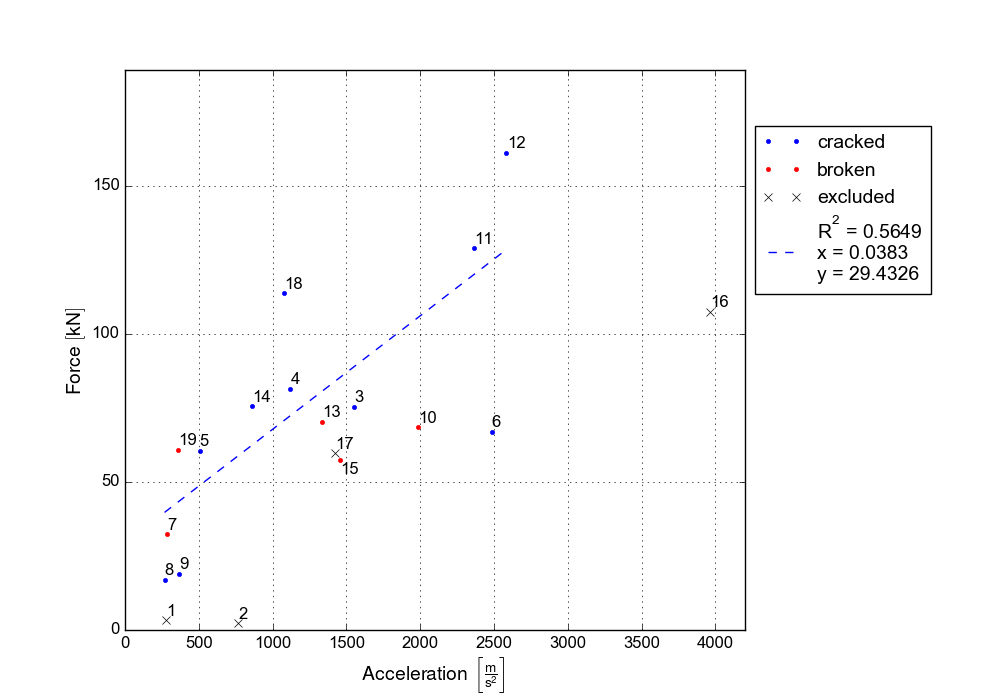
\includegraphics[width=0.95 \linewidth]{./diagram/Force_Acceleration}
    \caption{Force over acceleration}
    \label{fig:Acceleration_Force}
\end{figure}

\begin{figure}[p]
    \centering
    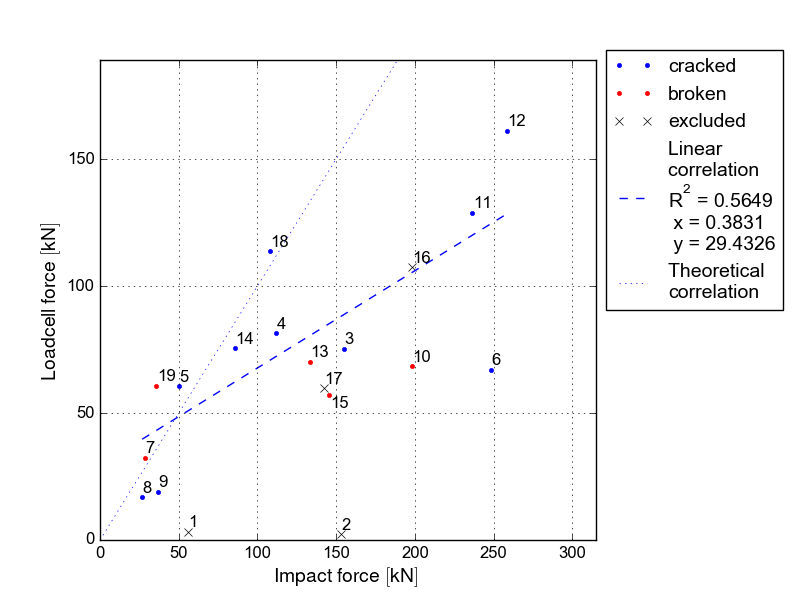
\includegraphics[width=0.95 \linewidth]{diagram/compare_impact_loadcell_force.png}
    \caption{Comparing the force of the impact to the force measured by the loadcells}
    \label{fig:compare_force}
\end{figure}

Force and acceleration correlate well. See \autoref{fig:Acceleration_Force}. Here broken and cracked samples both are very close to the curve. (10) 2018-11-29\_Rfrs\_75\_1,0 is the most obvious outlier because of the high acceleration. 
It was expected that force and acceleration would correlate slightly differently. The force of the impact of the drop weight can be calculated by multiplying the peak acceleration with the weight of the drop weight. According to basic physics: \(F = m * a\).  
As most test were conducted with the 100 kg drop weight the difference between drawing the impact force over the loadcell force and drawing the acceleration over the loadcell force is very small. See \autoref{fig:compare_force} and \autoref{fig:Acceleration_Force}.

Quite noticeable is that (16) 2019-04-16\_Rfrs\_75\_0,5 shifts from being an outlier to fitting very well with the other data. This sample was tested using the 50 kg drop weight. When using several different weights it appears that using the impact force instead of the acceleration might increase the comparability of results. More data is be needed to strength this assumption.

Theoretically  the impact force of the drop weight should be equal to the force measured by the loadcells. In \autoref{fig:compare_force} this theoretical line is presented by a blue dotted line.
In most cases the impact force is lower than the than the force measured by the load cells, the corresponding data points are below the line. %The reason is the energy that is dissipated by the formation of cracks. 
A possible short and simplified explanation would be that the sample starts vibrating when after the impact of the drop weight and these vibrations travel as waves through the sample to the load cells. If the sample forms cracks, some energy of the energy of these waves is absorbed. Therefore the waves are dampened by the time they reach the load cells. This model does not explain the samples where the load cells measure a higher force than the accelerometer does. The effect behind this is not yet understood and could be studied further. Examining the sample that are above or close to the line might yield clues. Sample (5) 2018-11-09\_Rfrs\_75\_0,5 is well above the line. The energy of the impact was 0,5 kJ which is below the critical energy. Probably little energy was lost to forming cracks as the sample was not very stressed.
Samples (7) 2018-12-04\_Rfrs\_50\_0,7, (8) 2018-12-04\_Rfrs\_50\_0,3 and (9) 2018-12-04\_Rfrs\_50\_0,3\_2 were all 50 mm thick. As previously noted, the thinner samples take a longer time to transfer the acceleration from the drop weight to the sample. This reduces the peak acceleration and therefore the impact force. This puts these samples closer to the line. The samples with a thickness of 100 mm, (10) 2018-12-10\_Rfrs\_100\_2,0, (11) 2018-12-10\_Rfrs\_100\_1,5	 and (12) 2018-12-10\_Rfrs\_100\_1,5\_2  are at a distance from the theoretical line still within the normal range. It appears that the thickness has limited influence on the acceleration experienced by the sample. See \autoref{fig:Acceleration_Thickness}.
Samples 	(18) 2019-08-19\_Rfrs+t\_75\_1,0 and (19) 2019-08-19\_Rfrs+t\_75\_1,0m2,0  were the sample. After the initial drop it was tested again. The TSL coat on the sample probably affected its behaviour. 
It appears that there is no simple explanation and that this behavior is dependant on several of parameters.


\begin{figure}
    \centering
    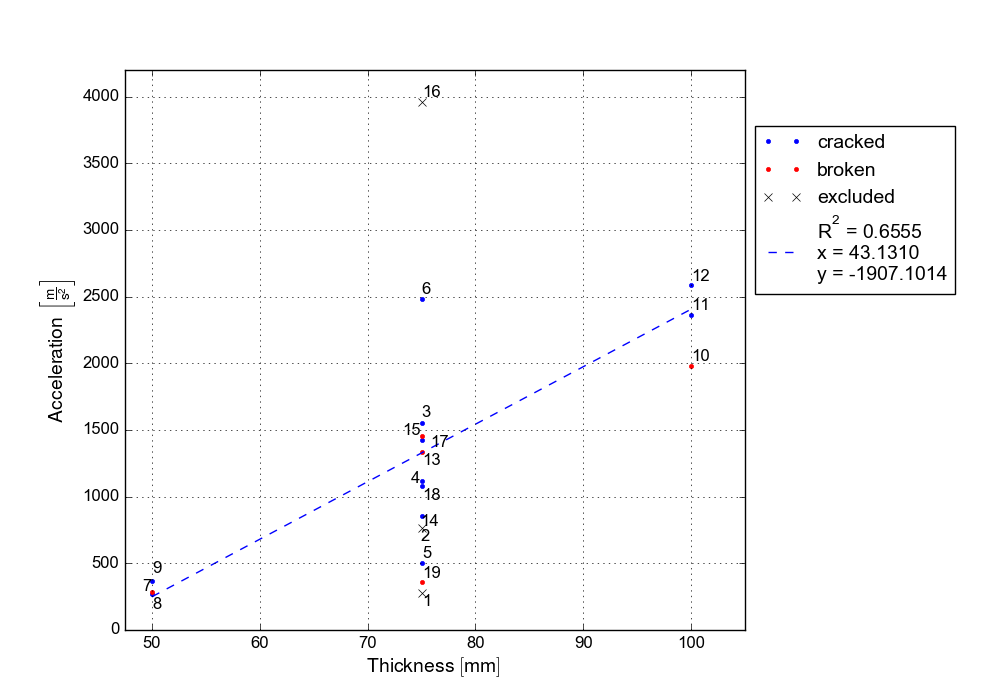
\includegraphics[width=0.95 \linewidth]{./diagram/Acceleration_Thickness}
    \caption{Acceleration over thickness}
    \label{fig:Acceleration_Thickness}
\end{figure}



%The force of the impact of the drop weight can be calculated from the acceleration measured by the accelerometer on the drop weight. 
 

\begin{figure}
    \centering
    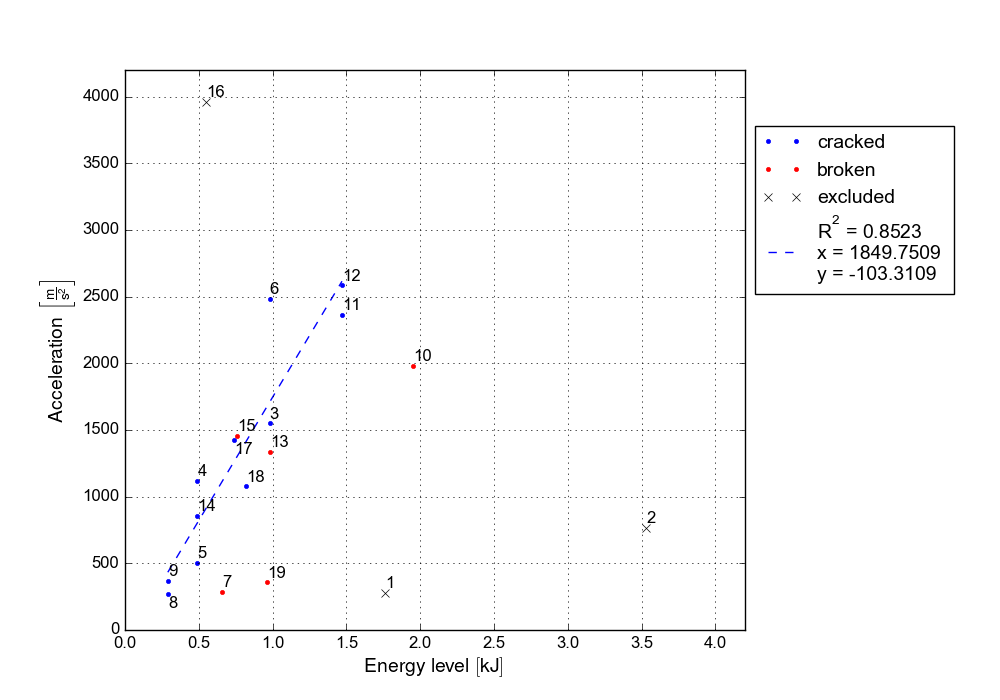
\includegraphics[width=0.95 \linewidth]{./diagram/Acceleration_Energy-level}
    \caption{Acceleration over energy levels}
    \label{fig:Acceleration_Energy-level}
\end{figure}

\begin{figure}
    \centering
    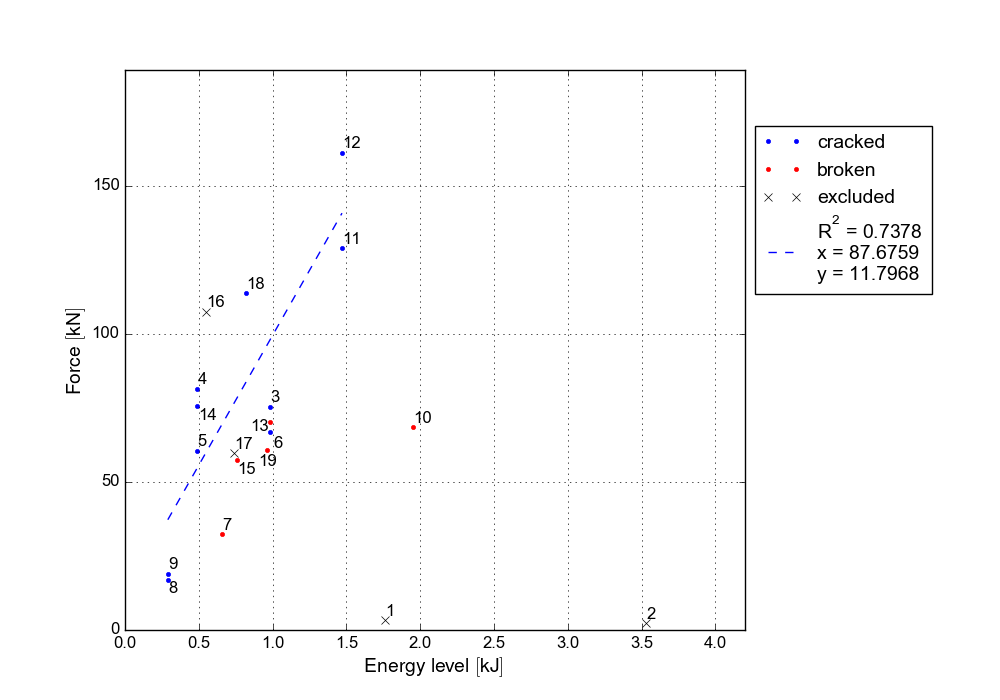
\includegraphics[width=0.95 \linewidth]{./diagram/Force_Energy-level}
    \caption{Force over energy level}
    \label{fig:Force_Energy-level}
\end{figure}

The accelerometer on the drop weight and the load cells correlate well with the energy level. See \autoref{fig:Acceleration_Energy-level} and \autoref{fig:Force_Energy-level}. These sensors are both indirect and measure what is going on inside of the sample. In both cases the broken samples mostly fit to the linear interpolated curve.  (4) 2018-12-10\_Rfrs\_100\_2,0 appears to be an outlier. Maybe because of the very high energy level. As long as the sample is not heavily overloaded it does not seem to influence the peak acceleration and the peak force if the sample breaks or cracks.




\begin{figure}
    \centering
    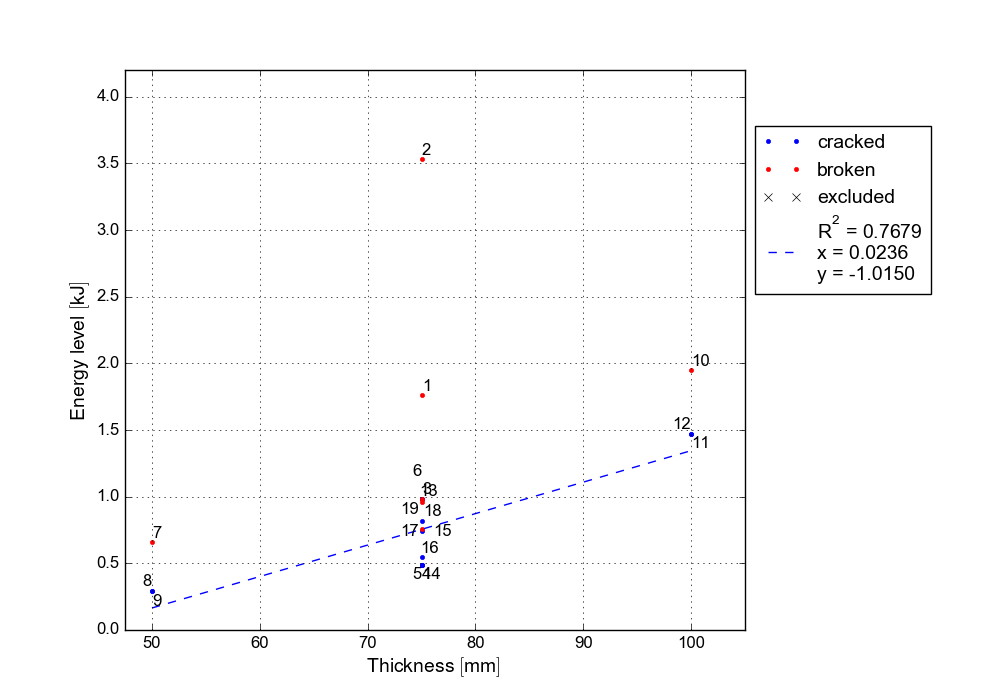
\includegraphics[width=0.95 \linewidth]{./diagram/Energy-level_Thickness}
    \caption{Energy level over thickness}
    \label{fig:Energy-level_Thickness}
\end{figure}

\begin{figure}
    \centering
    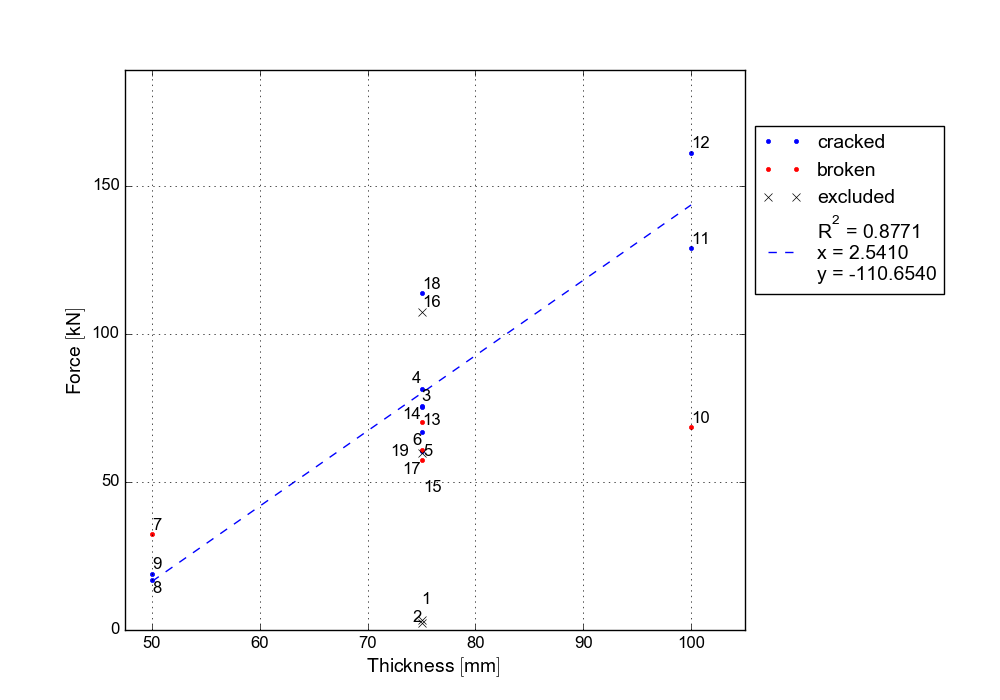
\includegraphics[width=0.95 \linewidth]{./diagram/Force_Thickness}
    \caption{Force over thickness}
    \label{fig:Force_Thickness}
\end{figure}

The sample thickness correlates well with the energy level and the acceleration of the drop weight. See \autoref{fig:Acceleration_Thickness} and \autoref{fig:Energy-level_Thickness}. When considering the curves, it seems the linear curve does fit but a poly nominal curve might fit better. There are not enough data points to draw such a curve satisfactorily. The acceleration again seems mostly unaffected by the outcome of the test. Both broken and cracked samples are grouped tightly together.

The thickness correlates extremely well with the force, see \autoref{fig:Force_Thickness}. Most of the broken samples fit quite well with the curve, again (4) 2018-12-10\_Rfrs\_100\_2,0  appears to be an outlier.

\begin{figure}
    \centering
    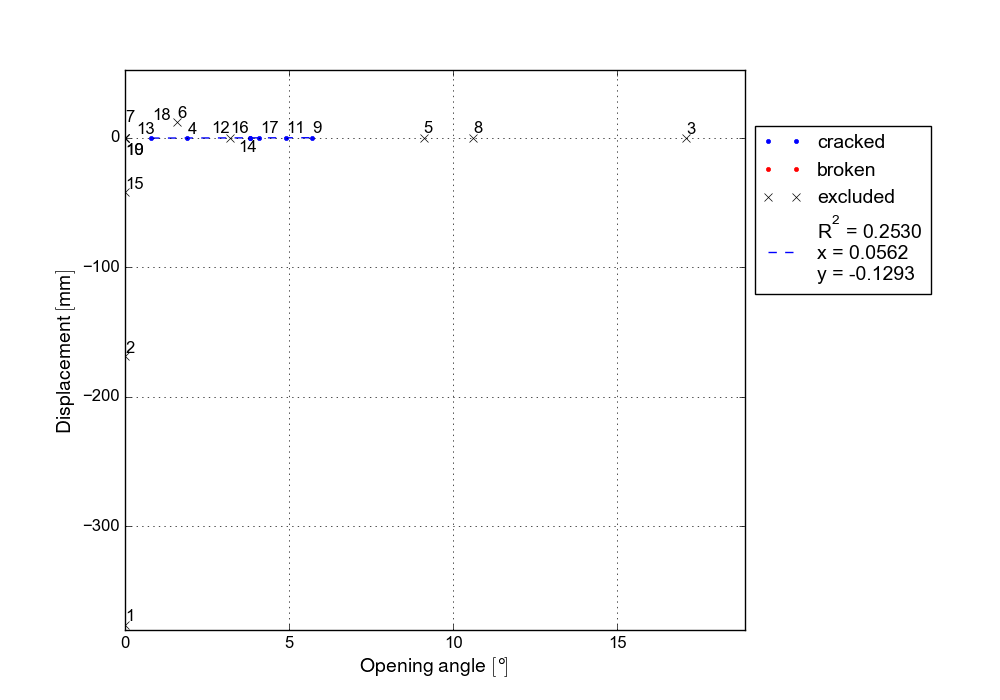
\includegraphics[width=0.95 \linewidth]{./diagram/Displacement_Opening-angle}
    \caption{Displacement over opening angle}
    \label{fig:Displacement_Opening-angle}
\end{figure}

\begin{figure}
    \centering
    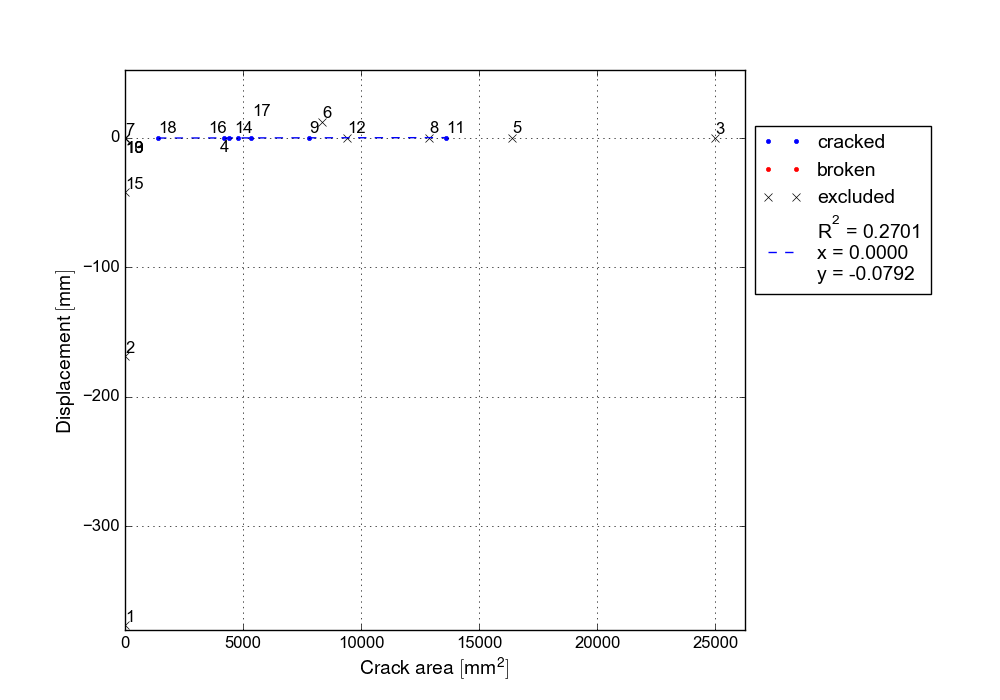
\includegraphics[width=0.95 \linewidth]{./diagram/Displacement_Crack-area}
    \caption{Displacement over crack area}
    \label{fig:Displacement_Crack-area}
\end{figure}

\begin{figure}
    \centering
    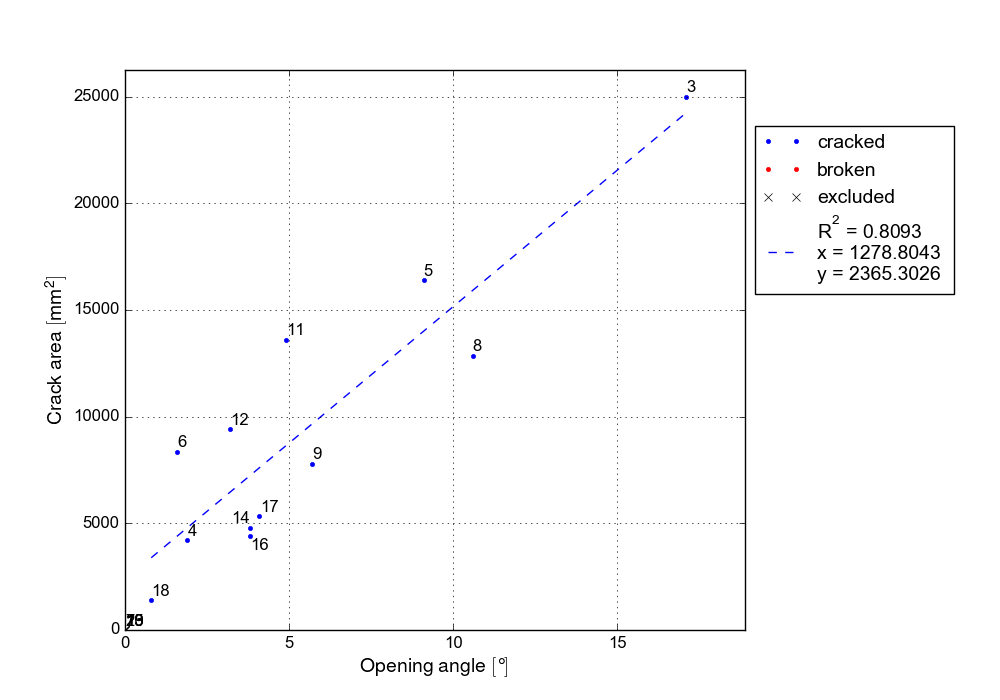
\includegraphics[width=0.95 \linewidth]{diagram/Crack-area_Opening-angle.png}
    \caption{Crack area over opening angle}
    \label{fig:Crack-area_Opening-angle}
\end{figure}

\begin{figure}
    \centering
    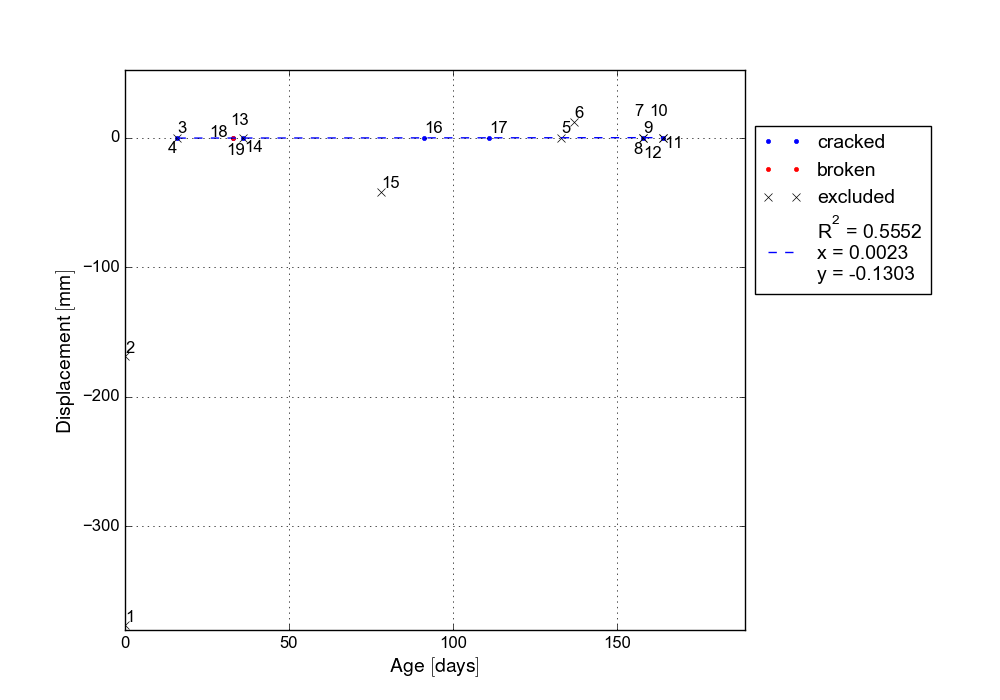
\includegraphics[width=0.95 \linewidth]{./diagram/Displacement_Age}
    \caption{Displacement over age of concrete}
    \label{fig:Displacement_Age}
\end{figure}

The displacement correlates well with the opening angle of the samples, see \autoref{fig:Displacement_Opening-angle}. Much better than with the crack area, see \autoref{fig:Displacement_Crack-area}. This is somewhat surprising as the opening angle is calculated from the crack area and correlates well with it. See \autoref{fig:Crack-area_Opening-angle}.

The displacement correlates very well with the age of the samples. See \autoref{fig:Displacement_Age}
It is likely that this correlation is just a coincidence due to the small number of data points.
The displacement correlates badly with the thickness of the samples and the peak force. With the energy level and the acceleration it does not correlate at all. This is surprising. It was expected that the amount of damage done to a sample is connected to the impact energy. Perhaps the actual cracking of a sample is more dependant on other factors. For example the crack might start at impurities or micro cracks. It´s outside of the scope of this thesis to make detailed observations of the formations of cracks. In order to be able to make such observations a high speed camera, with a very high frame rate would need to be set up underneath the sample, pointing upwards. At 5000 fps the formation of cracks appears to happen within one frame. A even higher frame rate would be necessary. Pointing the camera upwards at the sample would mean that the camera would have to be protected from debris somehow. Also such observations would face the same problem as the laser sensor readings: debris and dust obscuring the view. It might be worth considering after the impact table has been lifted and more space for equipment is available. 

%The strong correlation between energy level and shotcrete thickness is interesting. If arbitrarily deciding  all parameter pairs with R - values above 0,75 appear to be dependent on each other, the necessary sensor array shrinks significantly. Force and Acceleration both become redundant. Describing both crack area and crack opening angle is also not necessary.

%As long as the drop weight is kept consistent this assumption holds true. As described in %%%%REF 
%had to be removed, as the lighter drop weight changed the measured acceleration significantly. The impact velocity is directly dependent on the drop height.
%The weight of the drop weight appears to have more influence on the response of the sample than the actual energy input. This calls the test setup into question. It is theoretically possible that a sample performs very well when tested using a specific drop weight but poorly under another. Maybe this effect is less pronounced when testing large samples because the load will be distributed by a foam cushion.

%More tests with several drop tests are recommended to study this phenomenon. Perhaps it would be interesting to control the impact velocity.
%When controlling for drop weight the testing process can be streamlined significantly.

As long as the drop weight is held consistent many sensors correlate very strongly.

%%%%%%%%%%%%%%%%%%%%%%%%%%%%%%%%%%%%%%%%%%%%%%%%%%%%%%%%


\subsection{Streamlining the Testing Process}

A very aggressive approach to stream lining the testing process would be to cut the sensor array significantly. As shown in \autoref{fig:heat} all indirect sensors (loadcells, accelerometer on the drop weight and the drop height) correlate extremely well and the direct measurements (displacement and crack pattern) correlate only with each other. The displacement and other ways of mapping the damage of the sample appear to no correlate with the impact energy.

Therefore removing all sensors but the rotary encoder would be a way to reduce both preparatory work and post processing. The drop height is sufficient to estimate of the impact velocity, the force and the acceleration of the drop weight with an \(R^2\) value of > 0,70.

The high speed camera footage is aesthetically pleasing. But data collection is very failure prone, as became obvious when running the experiments. If it does work it is time intensive to evaluate. The results it yields are not very exact, as discussed previously. Therefore it appears redundant.

The accelerometers on the sample are also very vulnerable to failure and require a lot of preparation. They appear to influence the behaviour of the sample significantly. Either a different way of attaching them would be needed or they should be removed.

Tthe malfunctions of both the high speed camera and the accelerometers on the sample were both mostly caused by human error. A check list was implemented to help with this. Further measures to reduce human error would be to synchronise the accelerometers on the sample and the high speed camera with the data collection system. The question that poses itself is, if the data is worth the associated cost.

It was good to test with the full sensor array. Now there is data available that backs up the decision to reduce the sensor array.

When removing all the before mentioned sensors only two parameters still remain to be analysed. The drop height and the thickness of the panel.

\subsection{Correlation Between Thickness and Energy Absorption Capacity}
\label{ssec:energy}

When controlling for the drop weight, the survivable impact energy and the thickness of the panel appear to be linearly dependant. The parameters necessary to estimate the thickness at which a sample is sure to survive at a certain energy input are given in \autoref{fig:Energy-level_Thickness}. They can be summarised in a equation to enhance understanding. The round panels have a surface area of approximately 0,5 m. These equations are using rounded factor and have been modified to work per square meter of concrete.

See \autoref{equ:energy}.

%The slope is \(32,6203~\frac{\text{mm}}{\text{kJ}}\)  and the intercept is \(50,5644\) mm.  

\begin{equation}\label{equ:energy}
    \text{Necessary concrete thickness [mm]} = 16,5 ~\frac{\text{mm}}{\text{kJ}} * \text{Energy input [kJ]} + 25 ~\text{mm}
\end{equation}

 Through simple arithmetic the reverse equation can be deduced. See \autoref{equ:thickness}

\begin{equation} \label{equ:thickness}
    \text{Survivable energy [kJ]} = 0,047 ~\frac{\text{kJ}}{\text{mm}} * \text{Sample thickness [mm]} - 2,02 ~\text{kJ}
\end{equation}

The limitations of these equations are quite strict. They only apply for the type of concrete used in Kirunavaara mine with a thickness between 50 and 100 mm, when using a 100 kg as drop weight and using round panels. It should be mentioned that this is the linear interpolation of all samples that only cracked. Some samples broke at lower energy levels and some samples survived higher impacts.

\begin{table}
    \centering
    \begin{tabular}{ll}
    \toprule
    Thickness [mm]  & Energy [kJ]\\
    \midrule
    50             &   0,3 \\
    60              &   0,8 \\
    70             &   1,3 \\
    80              &   1,7 \\
    90             &   2,2 \\
    100              &   2,7 \\
    \bottomrule
    \end{tabular}
    \caption{Concrete thickness necessary to survive certain impact energy}
    \label{tab:estimate}
\end{table}

Using these equations it is possible to estimate the thickness of shotcrete required to survive various impacts. See \autoref{tab:estimate}. The current shotcrete thickness is 100 mm. This appears to be able to survive impact energies of 2,7 \(\frac{\text{kJ}}{\text{m}^\text{2}}\). %\textcite{Heal10} stated that FRS without mesh support fails at 1,5 to 2 \(\frac{\text{kJ}}{\text{m}^\text{2}}\) \textit{in - situ}.

%This design load appears to be significantly too high. 
Large sample tests are recommended to confirm these equations. \textcite{Potvin10} stated that 100 mm of FRS in drop tests usually achieve energy absorption capacities of between 5 - 10 \(\frac{\text{kJ}}{\text{m}^\text{2}}\). 
The results of the Kirunavaara test rig using round samples are significantly are lower than those of other test rigs. This should be taken into consideration when comparing results with other test rigs. A reason might be the shape of the drop weight.